%%%%%%%%%%%%%%%%%%%%%%%%%%%%%%%%%%%%%%%%%%%%%%%%%%%%%%%%%%%%%%%%%%%%%%%%%%%

\documentclass[a4paper,oneside,12pt]{article}
\usepackage{mystyle}

\begin{document}

\title{\Large\bf Applications of quadratic functions}
\author{%%
  Minh Van Nguyen \\
  \url{mvngu@gmx.com}
}
\date{\today}
\maketitle

\noindent
This document will show you how the quadratic function can be used in
a variety of situations.  The document consists of mostly worked
examples and exercises.  Carefully study the examples to understand
how the quadratic function is used in each case.  Wherever an equation
is given, you should attempt by yourself to derive the equation.  This
not only helps to solidify your understanding of a particular problem,
but also sharpens your problem solving skills.


%%%%%%%%%%%%%%%%%%%%%%%%%%%%%%%%%%%%%%%%%%%%%%%%%%%%%%%%%%%%%%%%%%%%%%%%%%%

\section{Length and width}

This section presents two examples from geometry where the quadratic
function can be used to determine lengths and widths of certain
geometric objects.

\begin{example}
\textbf{Fencing.}
\label{ex:fence_a_rectangular_region}
You want to install a fence around a rectangular region that has an
area of $7$ metres squared.  You want the length of the rectangular
region to be two metres longer than the width.  Calculate the width of
the region.
\end{example}

\begin{solution}
Whenever possible, you should first draw a picture to help you solve a
problem.  In this example, the rectangular region and its dimensions
can be illustrated as shown in
\Figure{fig:rectangular_region_7_metres_squared}.  Since the width of
the region is $w$ metres and its length is $w + 2$ metres, the area of
the region is $(w + 2)w$ metres squared.  However, you also know that
the region has an area of $7$~metres squared, which can be used to
give you the equation
%%
\begin{equation}
\label{eqn:rectangular_region_equation}
(w + 2)w
=
7.
\end{equation}

\begin{figure}[!htbp]
\centering
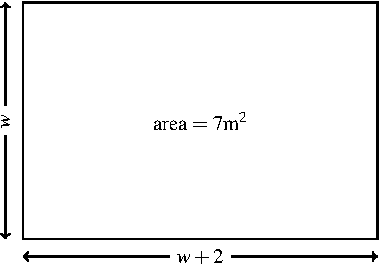
\includegraphics[scale=1.2]{image/09/rectangular-fence.pdf}
\caption{%%
  A rectangular region whose area is $7$ metres squared.  The width of
  the region is denoted $w$.
}
\label{fig:rectangular_region_7_metres_squared}
\end{figure}

Let's determine all values of $w$ that satisfy
\Equation{eqn:rectangular_region_equation}.  Expand the left-hand side
of \Equation{eqn:rectangular_region_equation} to get $w^2 + 2w = 7$.
Upon moving everything to the left-hand side, you end up with the
quadratic equation
%%
\begin{equation}
\label{eqn:rectangular_region_quadratic}
w^2 + 2w - 7
=
0.
\end{equation}
%%
Writing the left-hand side as $f(w) = w^2 + 2w - 7$,
\Equation{eqn:rectangular_region_quadratic} can also be written as
$f(w) = 0$.  This means that you want to determine all roots of
$f(w)$.  Before calculating the roots of $f(w)$, you investigate
whether $f(w)$ has a unique root, two different roots, or the graph of
$f(w)$ does not intersect the horizontal axis.  This is a job for the
discriminant.  The discriminant of $f(w)$ is $\Delta = 32$.  This is a
positive number so there exists at least one real value of $w$ that
solves \Equation{eqn:rectangular_region_equation}.  Using the
quadratic formula, the roots of $f(w)$ can be written as
$w = -1 \pm 2\sqrt{2}$.  One root of $f(w)$ is given by
\[
w_1
=
2\sqrt{2} - 1
\]
which is positive.  The other root is given by
\[
w_2
=
-2\sqrt{2} - 1
\]
which is negative.  You reject the number $w_2$ because the width of
the rectangular region cannot be a negative number.  To confirm your
decision to reject the root $w_2$, you sketch a graph of $f(w)$ as
shown in \Figure{fig:rectangular_region_quadratic_roots} and note that
$w_2$ is located on the negative half of the $w$-axis, i.e.~the
horizontal axis.  You conclude that the width of the rectangular
region is approximately $2\sqrt{2} - 1 \approx 1.8284$ metres long,
rounded to four decimal places.
\end{solution}

\begin{figure}[!htbp]
\centering
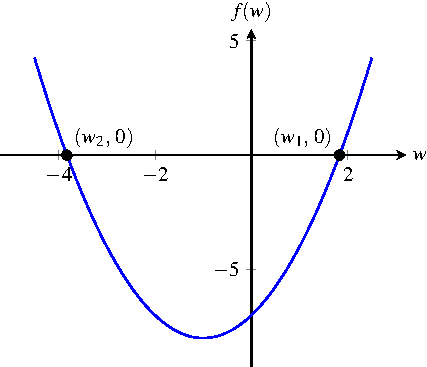
\includegraphics[scale=1.2]{image/09/a1-b2-cminus7.pdf}
\caption{%%
  Graph of the function $f(w) = w^2 + 2w - 7$.  The two dots indicate
  the two different roots of $f(w)$.
}
\label{fig:rectangular_region_quadratic_roots}
\end{figure}

\begin{exercise}
\label{ex:rectangular_region_discriminant}
In the solution of \Example{ex:fence_a_rectangular_region}, verify
that the discriminant is $\Delta = 32$.
\end{exercise}
%%
\ifbool{showSolution}{
\begin{solution}
In the equation $f(w) = w^2 + 2w - 7$, you have the values $a = 1$,
$b = 2$, and $c = -7$.  Use \Definition{def:discriminant} to see that
the discriminant of $f(w)$ is
%%
\begin{align*}
\Delta
&=
2^2 - 4(1)(-7) \\[4pt]
&=
4 + 28 \\[4pt]
&=
32
\end{align*}
%%
as required.
\end{solution}
}{}

\begin{exercise}
In the solution of \Example{ex:fence_a_rectangular_region}, verify
that the roots of $f(w)$ can be written as $w = -1 \pm 2\sqrt{2}$.
\end{exercise}
%%
\ifbool{showSolution}{
\begin{solution}
You have the equation $f(w) = w^2 + 2w - 7$, whose roots can be
calculated by using the quadratic formula.  The discriminant of $f(w)$
is known to be $\Delta = 32$, as verified in
\Exercise{ex:rectangular_region_discriminant}, so the roots are
%%
\begin{align*}
w
&=
\frac{
  -2 \pm \sqrt{\Delta}
}{
  2(1)
} \\[4pt]
&=
\frac{
  -2 \pm \sqrt{2 \times 4^2}
}{
  2
} \\[4pt]
&=
\frac{
  -2 \pm 4\sqrt{2}
}{
  2
} \\[4pt]
&=
\frac{
  2(-1 \pm 2\sqrt{2})
}{
  2
} \\[4pt]
&=
-1 \pm 2\sqrt{2}
\end{align*}
%%
as required.
\end{solution}
}{}

\begin{exercise}
A rectangle has a perimeter of $14$ centimetres and an area of $12$
centimetres squared.  Calculate the length and width of the
rectangle.
\end{exercise}

\ifbool{showSolution}{
\begin{solution}
Let $\ell$ and $w$ be the length and width, respectively, of the
rectangle.  The perimeter of the rectangle can be written as
%%
\begin{equation}
\label{eqn:rectangle_perimeter}
14
=
2(w + \ell)
\end{equation}
%%
and the area of the rectangle can be written as
%%
\begin{equation}
\label{eqn:rectangle_area}
12
=
w\ell.
\end{equation}
%%
Divide both sides of \Expression{eqn:rectangle_perimeter} by $2$ and
the perimeter of the rectangle can also be written as $7 = w + \ell$.
Solving the last equation for $\ell$ shows that the length of the
rectangle can be written as
%%
\begin{equation}
\label{eqn:rectangle_length}
\ell
=
7 - w.
\end{equation}
%%
Substitute \Expression{eqn:rectangle_length}
into~\eqref{eqn:rectangle_area} to write the area of the rectangle as
$12 = w(7 - w)$.  Use the distributive laws to expand the right-hand
side and you get $12 = -w^2 + 7w$.  Now move everything to the
left-hand side and you end up with
%%
\begin{equation}
\label{eqn:rectangle_area_quadratic}
w^2 - 7w + 12
=
0.
\end{equation}
%%
If you define the function $f(w) = w^2 - 7w + 12$, then
\Expression{eqn:rectangle_area_quadratic} can also be written as
$f(w) = 0$, which asks for all roots of $f(w)$.  That is, you want to
determine all values of $w$ such that
\Expression{eqn:rectangle_area_quadratic} is true.  This is equivalent
to determining all values of $w$ such that
\Expression{eqn:rectangle_area} is true.  The quadratic formula shows
that the roots of $f(w)$ are
%%
\begin{align*}
w
&=
\frac{
  -(-7) \pm \sqrt{(-7)^2 - 4(1)(12)}
}{
  2
} \\[4pt]
&=
\frac{7 \pm 1}{2}
\end{align*}
%%
both of which are positive.  One possible value for the width is
$w_1 = 4$ and the other possibility is $w_2 = 3$.

If the width is $w = 4$, substitute the latter expression into
\Expression{eqn:rectangle_length} to get a length of
$\ell = 7 - 4 = 3$.  Now you must check that a length of
$\ell = 3$ and a width of $w = 4$ will result in the required
perimeter and area for the rectangle.  Substitute the values
$\ell = 3$ and $w = 4$ into \Expression{eqn:rectangle_perimeter} and
you get
\[
14
=
2(4 + 3)
=
2 \times 7
\]
which is true.  Similarly, substitute the values $\ell = 3$ and
$w = 4$ into \Expression{eqn:rectangle_area} and you have
\[
12
=
4 \times 3
\]
which is also true.  Therefore if the length and width are
$\ell = 3$ and $w = 4$ centimetres, respectively, then you obtain the
required perimeter and area for the rectangle.

If the width is $w = 3$ centimetres, you can repeat the above process
to determine the corresponding length.  You then check your answer by
substitution back into
\Expressions{eqn:rectangle_perimeter}{eqn:rectangle_area}.
\end{solution}
}{}

\begin{example}
\label{ex:running_ants}
\textbf{Ant race.}
Two ants are next to each other.  Ant $A$ runs eastward at a rate of
two centimetres per second.  After one second since ant $A$ started
running, ant $B$ runs northward also at the same rate.  How long since
ant $A$ started running does it take for both ants to be five
centimetres apart?
\end{example}

\begin{solution}
As in \Example{ex:fence_a_rectangular_region}, you should first draw a
picture that can help you in solving the problem.  Denote by $t$ the
time in seconds and use $t$ to represent the amount of time that ant
$A$ runs.  Since ant $A$ runs in the eastern direction at two
centimetres per second, after $t$ seconds the ant would have covered a
horizontal distance of $2t$ centimetres.  When ant $A$ starts running,
ant $B$ is still at the starting position and must wait one second
before it starts to run in the northern direction.  The amount of time
that ant $B$ runs is one second less than the amount of time that ant
$A$ runs.  In other words, the duration of time that ant $B$ runs can
be written as $t - 1$ seconds, after which the ant would have
travelled a vertical distance of $2(t - 1)$ centimetres.  The
situation is illustrated in \Figure{fig:running_ants_triangle}.

\begin{figure}[!htbp]
\centering
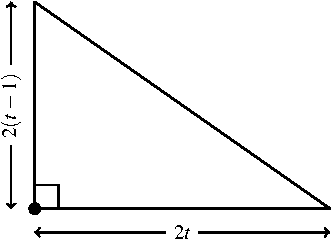
\includegraphics[scale=1.2]{image/09/running-ants.pdf}
\caption{%%
  A right-angled triangle that represents the directions in which two
  ants run.  The dot indicates the starting position of the ants.  The
  variable $t$ denotes time in seconds.  After $t$ seconds, the
  distance between the ants is represented by the length of the
  hypotenuse.
}
\label{fig:running_ants_triangle}
\end{figure}

Let's now formulate the problem as an equation.  The horizontal and
vertical distances travelled by both ants can be represented as the
base and height, respectively, of the right-angled triangle in
\Figure{fig:running_ants_triangle}.  After $t$ seconds have passed,
the distance between the ants is represented by the length of the
hypotenuse of the triangle.  Using Pythagoras' theorem, the problem
can be formulated as the quadratic equation
%%
\begin{equation}
\label{eqn:running_ants_quadratic_equation}
8t^2 - 8t + 4
=
25.
\end{equation}

The problem now is to determine all values of $t$ that satisfy
\Equation{eqn:running_ants_quadratic_equation}.  Note that the
equation can also be written as
\[
8t^2 - 8t - 21
=
0.
\]
Writing $f(t) = 8t^2 - 8t - 21$,
\Equation{eqn:running_ants_quadratic_equation} is equivalent to the
equation $f(t) = 0$, hence the values of $t$ that satisfy
\Equation{eqn:running_ants_quadratic_equation} are the same as the
roots of $f(t)$.  The quadratic formula shows that the roots of $f(t)$
are
%%
\begin{equation}
\label{eqn:running_ants_roots}
t_1
=
\frac{1}{2}
+
\frac{\sqrt{46}}{4}
%%
\qquad
\text{and}
\qquad
%%
t_2
=
\frac{1}{2}
-
\frac{\sqrt{46}}{4}.
\end{equation}
%%
You reject the root $t_2$ because it is negative.  A negative value of
time does not make sense in the context of the problem.  Therefore the
ants would be five centimetres apart after approximately
$\frac{1}{2}
+
\frac{\sqrt{46}}{4}
\approx
2.1956$
seconds~(rounded to four decimal places) since ant $A$ started running.
\end{solution}

\begin{exercise}
Explain why \Example{ex:running_ants} can be represented as
\Equation{eqn:running_ants_quadratic_equation}.
\end{exercise}
%%
\ifbool{showSolution}{
\begin{solution}
From \Figure{fig:running_ants_triangle} you know that after $t$
seconds, ant $A$ would have travelled $2t$ centimetres and ant $B$
would have travelled $2(t - 1)$ centimetres.  These numbers are the
base and height, respectively, of a right-angled triangle.  After $t$
seconds, the distance between the ants is represented by the  length
of the hypotenuse in \Figure{fig:running_ants_triangle}.  You want to
know when the ants are $5$ centimetres apart, so the hypotenuse is $5$
centimetres.  By Pythagoras' theorem, the three sides of the
right-angled triangle are related by the equation
\[
(2t)^2 + \bigparen{2 (t - 1)}^2
=
5^2.
\]
Upon expanding the parentheses, the equation can be written as
\[
4t^2 + (2t - 2)^2
=
25.
\]
Expand the remaining pair of parentheses to get
\[
4t^2 + 4t^2 - 8t + 4
=
25.
\]
After collecting like terms, you end up with
\Equation{eqn:running_ants_quadratic_equation}.
\end{solution}
}{}

\begin{exercise}
In the solution to \Example{ex:running_ants}, verify that the roots of
$f(t)$ are those given by~\eqref{eqn:running_ants_roots}.
\end{exercise}
%%
\ifbool{showSolution}{
\begin{solution}
You have the quadratic function $f(t) = 8t^2 - 8t - 21$.  Using the
quadratic formula, the roots of $f(t)$ are
%%
\begin{align*}
t
&=
\frac{
  -(-8) \pm \sqrt{(-8)^2 - 4(8)(-21)}
}{
  2(8)
} \\[4pt]
&=
\frac{
  8 \pm \sqrt{736}
}{
  16
} \\[4pt]
&=
\frac{
  8 \pm \sqrt{4^2 \times 2 \times 23}
}{
  16
} \\[4pt]
&=
\frac{
  8 \pm 4\sqrt{46}
}{
  16
} \\[4pt]
&=
\frac{
  4 \parenthesis*{2 \pm \sqrt{46}}
}{
  4^2
} \\[4pt]
&=
\frac{
  2 \pm \sqrt{46}
}{
  4
} \\[4pt]
&=
\frac{1}{2}
\pm
\frac{\sqrt{46}}{4}
\end{align*}
%%
which are the same as those given by~\eqref{eqn:running_ants_roots}.
\end{solution}
}{}


%%%%%%%%%%%%%%%%%%%%%%%%%%%%%%%%%%%%%%%%%%%%%%%%%%%%%%%%%%%%%%%%%%%%%%%%%%%

\section{Largest or smallest}

This section considers two optimisation problems.  Such problems
require you to maximise or minimise a particular function.  In the
context of a quadratic function, the optimised value of the function
is the function's vertex.

\begin{example}
\label{eg:largest_area_rectangle}
\textbf{Largest area.}
A rectangle has a perimeter of ten metres.
%%
\begin{packedenum}
\item\label{subex:largest_area_perimeter_area}
  Derive a function for the area of the rectangle.

\item\label{subex:largest_area_of_rectangle}
  Calculate the largest area that the rectangle can have.
\end{packedenum}
\end{example}

\begin{solution}
\solutionpart{subex:largest_area_perimeter_area}
As in \Examples{ex:fence_a_rectangular_region}{ex:running_ants}, you
should draw a picture to help you solve the problem.  Let $\ell$ and
$w$ be the length and width, respectively, of the rectangle.  Since
the rectangle has a perimeter of ten metres, the equation for the
perimeter can be written as
\[
2\ell + 2w
=
10
\]
and thus the length can be written as $\ell = 5 - w$.  The length and
width of the rectangle are illustrated in
\Figure{fig:largest_area_rectangle}.  Using the information from
\Figure{fig:largest_area_rectangle}, the area of the rectangle can be
written as the function
\[
f(w)
=
(5 - w)w
\]
which after expansion becomes $f(w) = -w^2 + 5w$.

\begin{figure}[!htbp]
\centering
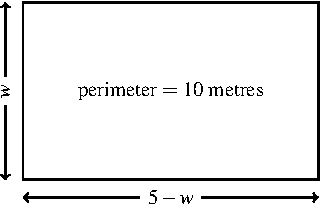
\includegraphics[scale=1.2]{image/09/largest-area.pdf}
\caption{%%
  A rectangle whose perimeter is ten metres.  The width is denoted as
  $w$ and the length is $5 - w$.
}
\label{fig:largest_area_rectangle}
\end{figure}

\begin{figure}[!htbp]
\centering
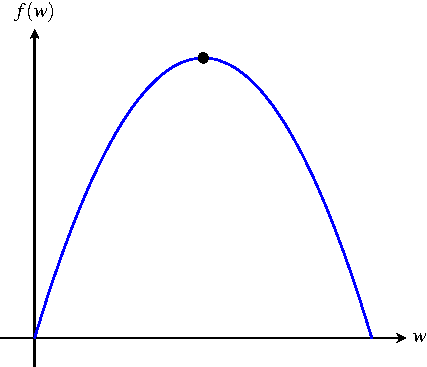
\includegraphics[scale=1.2]{image/09/rectangle-area.pdf}
\caption{%%
  The area $f(w) = (5 - w) w$ of a rectangle as a function of its
  width $w$.  The vertex of the parabola is the highest point in the
  graph of $f(w)$.  Here, the vertex is also the point at which the
  value of $f(w)$, or the area, is largest.
}
\label{fig:largest_area_graph_parabola}
\end{figure}

\solutionpart{subex:largest_area_of_rectangle}
\Figure{fig:largest_area_graph_parabola} shows a graph of the function
$f(w)$.  Note the highest point in the graph.  The horizontal
coordinate~(i.e.~the value of $w$) gives you the width of the
rectangle.  The vertical coordinate~(i.e.~the value of $f(w)$) gives
you the corresponding area of the rectangle.  So the largest area of
the rectangle occurs at the vertex in the graph of $f(w)$.  The
horizontal coordinate of the vertex is
\[
w
=
\frac{5}{2}.
\]
In other words, the largest value of the function $f(w)$ occurs when
the width is $w = 5 / 2 = 2.5$ metres.  What about the actual value of
$f(w)$?  Substitute $w = 5 / 2$ into $f(w)$ to get
\[
f(5/2)
=
\frac{25}{4}.
\]
This tells you that the largest area the rectangle can have is
$25 / 4 = 6.25$ metres squared.
\end{solution}

\begin{exercise}
In \Example{eg:largest_area_rectangle}, explain why the length of the
rectangle can be written as $\ell = 5 - w$.
\end{exercise}

\ifbool{showSolution}{
\begin{solution}
Note that the perimeter of the rectangle can be written as
\[
2\ell + 2w
=
10
\]
where $\ell$ and $w$ are the length and width, respectively, of the
rectangle.  You can also write the last equation as
$2(\ell + w) = 10$, which can be simplified to $\ell + w = 5$.  The
length of the rectangle can now be written as $\ell = 5 - w$.
\end{solution}
}{}

\begin{exercise}
In \Example{eg:largest_area_rectangle}, verify that the vertex of the
function $f(w)$ occurs at the point
$\tuple{\frac{5}{2}}{\frac{25}{4}}$.
\end{exercise}

\ifbool{showSolution}{
\begin{solution}
The horizontal coordinate of the vertex is
%%
\begin{align*}
w
&=
-\frac{5}{2(-1)} \\[4pt]
&=
\frac{-5}{-2} \\[4pt]
&=
\frac{5}{2}.
\end{align*}
%%
To get the vertical coordinate of the vertex, substitute $w = 5 / 2$
into $f(w)$ to get
%%
\begin{align*}
f(5/2)
&=
\parenthesis*{5 - \frac{5}{2}} \frac{5}{2} \\[4pt]
&=
\parenthesis*{\frac{10}{2} - \frac{5}{2}} \frac{5}{2} \\[4pt]
&=
\frac{5}{2} \times \frac{5}{2} \\[4pt]
&=
\frac{25}{4}
\end{align*}
%%
as required.
\end{solution}
}{}

\begin{example}
\label{eg:smallest_product}
\textbf{Smallest product.}
Let $x$ and $y$ be two numbers such that when you subtract $y$ from
$x$ you get $1$.  Determine the smallest value of the product $xy$.
\end{example}

\begin{solution}
From the statement of the problem, you have the equation
\[
x - y
=
1
\]
and so $y$ can be written as $y = x - 1$.  The product of $x$ and $y$
can be written as the quadratic function $f(x) = x^2 - x$, a graph of
which is shown in \Figure{fig:graph_smallest_product}.

\begin{figure}[!htbp]
\centering
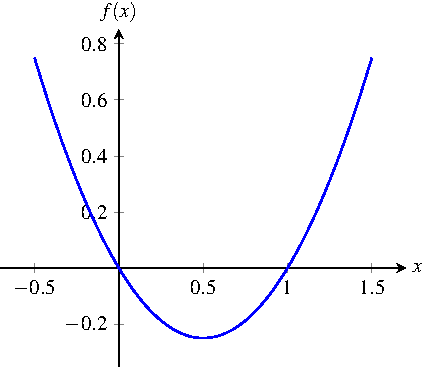
\includegraphics[scale=1.2]{image/09/smallest-product.pdf}
\caption{%%
  A graph of the function $f(x) = x^2 - x$, whose vertex is its lowest
  point.
}
\label{fig:graph_smallest_product}
\end{figure}

As $f(x)$ is a function that represents the product of $x$ and $y$,
the graph in \Figure{fig:graph_smallest_product} shows that the
smallest value of the product $xy$ occurs at the vertex of $f(x)$.
The horizontal coordinate of the vertex is
\[
x
=
\frac{1}{2}.
\]
Hence the vertical coordinate of the vertex is
\[
f(1/2)
=
-\frac{1}{4}.
\]
This tells you that the smallest value of the product $xy$ is
$-\frac{1}{4}$ and this least value occurs when $x = 1/2$.
\end{solution}

\begin{exercise}
In \Example{eg:smallest_product}, explain why $y$ can be written as
$y = x - 1$.
\end{exercise}

\ifbool{showSolution}{
\begin{solution}
You have the equation $x - y = 1$.  Move everything to the left-hand
side and you get $x - y - 1 = 0$.  Upon moving $y$ to the right-hand
side you end up with $x - 1 = y$.
\end{solution}
}{}

\begin{exercise}
In \Example{eg:smallest_product}, show that the product $xy$ can be
written as the function $f(x) = x^2 - x$.
\end{exercise}

\ifbool{showSolution}{
\begin{solution}
Since $y = x - 1$, the product $xy$ can be written as
\[
xy
=
x(x - 1).
\]
Use the distributive laws to expand the right-hand side and you get
$x^2 - x$.
\end{solution}
}{}

\begin{exercise}
In \Example{eg:smallest_product}, verify that the vertex of the
function $f(x) = x^2 - x$ is the point
$\tuple{\frac{1}{2}}{-\frac{1}{4}}$.
\end{exercise}

\ifbool{showSolution}{
\begin{solution}
The horizontal coordinate of the vertex of $f(x)$ is
%%
\begin{align*}
x
&=
-\frac{-1}{2(1)} \\[4pt]
&=
\frac{1}{2}.
\end{align*}
%%
The vertical coordinate of the vertex is
%%
\begin{align*}
f(1/2)
&=
\parenthesis*{\frac{1}{2}}^2 - \frac{1}{2} \\[4pt]
&=
\frac{1}{4} - \frac{2}{4} \\[4pt]
&=
\frac{1 - 2}{4} \\[4pt]
&=
-\frac{1}{4}
\end{align*}
%%
as required.
\end{solution}
}{}


%%%%%%%%%%%%%%%%%%%%%%%%%%%%%%%%%%%%%%%%%%%%%%%%%%%%%%%%%%%%%%%%%%%%%%%%%%%

\section{Free fall}

This section considers an example from physics.  You throw a small
ball straight up into the air.  The ball travels upward in a straight
line for some time, reaches a maximum height, and then falls to the
ground.  Other than throwing the ball upward, you do not interfere
with the movement of the ball, but allow the forces of gravity and air
drag~(air resistance) to act on the ball.  In many cases, the force of
air drag can be ignored.  For now you only need to take into account
the force of gravity.  When the ball is allowed to move vertically as
described above, the motion of the ball is an example of
\emph{free fall}.

The position of the ball changes with time.  But precisely in what
way?  To analyse the position of the ball, let's make various
assumptions.  Denote by $t$ the time in seconds and let $f(t)$ be the
height in metres of the ball.  The \emph{initial height} of the ball
is the ball's height above ground level before the ball moves upward.
When you hold the ball in your hand just before you throw it upward,
the initial height of the ball is the distance~(in metres) from your
hand to the ground.  If the ball is on the ground before it moves
upward, its initial height is zero metres.  Let $h$ be the initial
height of the ball.  The \emph{initial velocity} of the ball is the
speed in metres per second with which the ball is thrown upward.
Denote the initial velocity of the ball by $v$.  The force of gravity
acts on the ball in a downward manner.  This is because gravity tends
to pull an object downward towards the centre of the Earth.  The force
of gravity is usually written as $g$ and its value is the constant of
$9.8$ metres per second squared.  To analyse the position of the ball,
you must take into account the initial height of the ball, the upward
distance it travels as time passes, and the downward force of gravity.
The position of the ball above ground level can be approximated by the
quadratic function
%%
\begin{equation}
\label{eqn:position_of_object_under_free_fall}
f(t)
=
-\frac{1}{2} gt^2 + vt + h.
\end{equation}

\begin{example}
\label{ex:spring_ball}
\textbf{Boing boing.}
A spring is located at ground level and can shoot a ball upward at an
initial velocity of $10$ metres per second.
%%
\begin{packedenum}
\item\label{ex:spring_ball_graph}
  Write a function for the position of the ball and graph the
  function.

\item\label{ex:spring_ball_time_to_maximum_height}
  Determine the amount of time~(in seconds) required for the ball to
  reach maximum height.  Calculate the maximum height~(in metres) that
  the ball reaches.

\item\label{ex:spring_ball_time_hit_ground}
  When will the ball reach the ground?
\end{packedenum}
\end{example}

\begin{solution}
\solutionpart{ex:spring_ball_graph}
You know that the force of gravity is $g = 9.8$ metres per second
squared.  The initial velocity is $v = 10$ metres per second.  Since
the spring is located at ground level, let's assume that the initial
height of the ball is $h = 0$ metres.  Substitute these values into
\Equation{eqn:position_of_object_under_free_fall} and simplify the
result to get
\[
f(t)
=
-\frac{49}{10}t^2 + 10t
\]
whose graph is shown in \Figure{fig:spring_ball_graph}.  This is a
rough sketch that illustrates three points on which you should
concentrate.  First is the point at the origin $\tuple{0}{0}$ that
tells you the initial height of the ball at time $t = 0$ before the
ball is shot upward.  Next is the vertex of the function $f(t)$, which
in this example is the highest point $\tuple{a}{f(a)}$ of the graph of
$f(t)$.  The vertex $\tuple{a}{f(a)}$ tells you that the ball reaches
its maximum height of $f(a)$ metres above the ground at time $t = a$
seconds after being shot upward by the spring.  The third point
$\tuple{b}{0}$ tells you approximately how long the ball is in the air
before it lands on the ground.  You do not yet know the values of $a$
and $b$.  This is just a rough sketch to help you understand the
example.

\begin{figure}[!htbp]
\centering
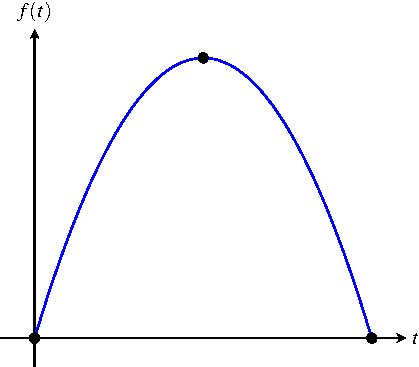
\includegraphics[scale=1.2]{image/09/spring-ball.pdf}
\caption{%%
  The height of a ball as a function of time.  Here, time $t$ is
  measured in seconds and the height $f(t)$ of the ball is measured in
  metres above the ground.
}
\label{fig:spring_ball_graph}
\end{figure}

\solutionpart{ex:spring_ball_time_to_maximum_height}
You know that the vertex~(i.e. highest point) of the graph of $f(t)$
occurs at $t = 50/49$.  This means that the ball reaches its maximum
height above the ground at approximately $t = 50/49 \approx 1.0204$
seconds~(rounded to four decimal places) after being shot up by the
spring.  The maximum height that the ball reaches is
$f(50 / 49) = 250 / 49$, which is approximately $5.1020$ metres above
the ground, rounded to four decimal places.

\solutionpart{ex:spring_ball_time_hit_ground}
You can use the quadratic formula to calculate the time at which the
ball hits the ground.  However, the following is a simple method that
does not use the quadratic formula.  Note that the function $f(t)$ can
be factorised as
%%
\begin{align*}
f(t)
&=
-\frac{49}{10} t^2 + 10t \\[4pt]
&=
\parenthesis*{-\frac{49}{10} t + 10} t \\[4pt]
&=
\parenthesis*{10 - \frac{49}{10} t} t.
\end{align*}
%%
Since the roots of $f(t)$ are those values of $t$ such that the
equation $f(t) = 0$ is true, this is the same as determining the
values of $t$ such that the following equation is true:
%%
\begin{equation}
\label{eqn:spring_ball_equation_factored}
\parenthesis*{10 - \frac{49}{10} t} t
=
0.
\end{equation}
%%
Equation~\eqref{eqn:spring_ball_equation_factored} is true when
$t = 0$.  However, when $t = 0$ the ball is at its initial height of
zero metres above ground level and so the point $\tuple{0}{0}$ is the
starting position of the ball when it is initially on the ground.  In
other words, you can ignore the root $t = 0$ of $f(t)$.  Let's
consider the other factor $10 - \frac{49}{10} t$.  If you have
$10 - \frac{49}{10} t = 0$, then
\Equation{eqn:spring_ball_equation_factored} will also be true.  Now
you must solve the equation $10 - \frac{49}{10} t = 0$ for $t$.  Doing
so gives you the root $t = 100 / 49$.  Therefore the ball will reach
the ground at approximately $t = 100 / 49 \approx 2.0408$ seconds
after being shot up by the spring.
\end{solution}

\begin{exercise}
You will verify the solution of \Example{ex:spring_ball}.
%%
\begin{packedenum}
\item\label{subex:spring_ball_height_function}
  Show that the height of the ball can be written as
  $f(t) = -\frac{49}{10} t^2 + 10t$.

\item\label{subex:spring_ball_highest_point}
  Show that the ball reaches its maximum height at $t = 50 / 49$
  seconds after being shot up.  Also show that the maximum height of
  the ball is $f(50 / 49) = 250 / 49$ metres above the ground.

\item\label{subex:spring_ball_quadratic_formula}
  Use the quadratic formula to calculate the roots of $f(t)$.
\end{packedenum}
\end{exercise}
%%
\ifbool{showSolution}{
\begin{solution}
\solutionpart{subex:spring_ball_height_function}
You know that the force of gravity is $g = 9.8 = 49/5$ metres per
second squared, the initial velocity of the ball is $v = 10$ metres
per second, and the initial height of the ball is $h = 0$ metres above
ground level.  Substitute these values into
\Equation{eqn:position_of_object_under_free_fall} to obtain
%%
\begin{align*}
f(t)
&=
-\frac{49}{5} \times \frac{1}{2} t^2 + 10t + 0 \\[4pt]
&=
-\frac{49}{10} t^2 + 10t.
\end{align*}

\solutionpart{subex:spring_ball_highest_point}
The horizontal coordinate of the vertex of $f(t)$ is
%%
\begin{align*}
t
&=
-\frac{10}{2 \times \parenthesis*{-\frac{49}{10}}} \\[4pt]
&=
\frac{10}{\frac{49}{5}} \\[4pt]
&=
10 \times \frac{5}{49} \\[4pt]
&=
\frac{50}{49}.
\end{align*}
%%
Then the vertical coordinate of the vertex is
%%
\begin{align*}
f(50 / 49)
&=
-\frac{49}{10} \parenthesis*{\frac{50}{49}}^2
+
10\parenthesis*{\frac{50}{49}} \\[4pt]
&=
-\frac{49}{10} \times \frac{50^2}{49^2}
+
\frac{10 \times 50}{49} \\[4pt]
&=
-\frac{5 \times 50}{49}
+
\frac{10 \times 50}{49} \\[4pt]
&=
\frac{
  50(10 - 5)
}{
  49
} \\[4pt]
&=
\frac{
  250
}{
  49
}.
\end{align*}
%%

\solutionpart{subex:spring_ball_quadratic_formula}
Using the quadratic formula results in
%%
\begin{align*}
t
&=
\frac{
  -(10) \pm \sqrt{10^2 - 4\parenthesis*{-\frac{49}{10}} (0)}
}{
  2 \parenthesis*{-\frac{49}{10}}
} \\[4pt]
&=
\frac{
  -10 \pm \sqrt{10^2}
}{
  -\frac{49}{5}
} \\[4pt]
&=
\frac{
  -10 \pm 10
}{
  -\frac{49}{5}
}.
\end{align*}
%%
The roots of $f(t)$ are
\[
t_1
=
\frac{
  -10 + 10
}{
  -\frac{49}{5}
}
=
0
%%
\qquad
\text{and}
\qquad
%%
t_2
=
\frac{
  -10 - 10
}{
  -\frac{49}{5}
}
=
\frac{100}{49}.
\]

\end{solution}
}{}

\begin{exercise}
You hold a small marble in your right hand.  The distance from your
right hand to the ground is one metre.  You throw the marble upward at
an initial velocity of eight metres per second.  Suppose that the
marble travels in a straight line upward, then falls to the ground
after a certain amount of time.
%%
\begin{packedenum}
\item\label{subprob:marble_distance_function}
  Write a function for the position~(in metres above the ground) of
  the marble.

\item\label{subprob:marble_time_to_land}
  After you have thrown the marble upward, determine the amount of
  time~(in seconds) required for the marble to reach the ground.

\item\label{subprob:marble_maximum_height}
  Calculate the maximum height~(in metres above the ground) that the
  marble reaches.
\end{packedenum}
\end{exercise}

\ifbool{showSolution}{
\begin{solution}
\solutionpart{subprob:marble_distance_function}
The initial height~(above the ground) of the marble is $h = 1$ metre
and the initial velocity of the marble is $v = 8$ metres per second.
Substitute these values into
\Expression{eqn:position_of_object_under_free_fall} and you obtain
\[
f(t)
=
-\frac{1}{2}gt^2 + 8t + 1.
\]
Here $g = 9.8$ metres per second squared is the force of gravity, $t$
represents time in seconds, and $f(t)$ is a function of the height~(in
metres above the ground) of the marble.

\solutionpart{subprob:marble_time_to_land}
The amount of time required for the marble to reach the ground is
equivalent to the roots of $f(t)$.  The quadratic formula shows that
the roots of $f(t)$ are given by
%%
\begin{align*}
t
&=
\frac{
  -8
  \pm
  \sqrt{8^2 - 4\parenthesis*{-\frac{1}{2}g}(1)}
}{
  2\parenthesis*{-\frac{1}{2}g}
} \\[4pt]
&=
\frac{
  -8
  \pm
  \sqrt{64 + 2g}
}{
  -g
}.
\end{align*}
%%
One root is
\[
t_1
=
\frac{
  -8
  -
  \sqrt{64 + 2g}
}{
  -g
}
\approx
1.7493
\]
and the other root is
\[
t_2
=
\frac{
  -8
  +
  \sqrt{64 + 2g}
}{
  -g
}
\approx
-0.1167
\]
both rounded to four decimal places.  You reject the root $t_2$
because it does not make sense in the context of the problem.
Conclude that after you have thrown the marble upward, the marble
requires approximately $1.7493$ seconds to reach the ground.

\solutionpart{subprob:marble_maximum_height}
The maximum height~(in metres above the ground) that the marble
reaches is equivalent to the vertex of $f(t)$.  The horizontal
coordinate of the vertex is
\[
t
=
\frac{
  -8
}{
  2\parenthesis*{-\frac{1}{2}g}
}
=
\frac{8}{g}
\]
and the vertical coordinate of the vertex is
%%
\begin{align*}
f(8/g)
&=
-\frac{1}{2}g\parenthesis*{\frac{8}{g}}^2
+
8\parenthesis*{\frac{8}{g}}
+
1 \\[4pt]
&=
\frac{32}{g} + 1.
\end{align*}
%%
In other words, the marble reaches a maximum height of approximately
$f(8/g) \approx 4.2653$ metres above the ground, rounded to four
decimal places.  This occurs at approximately $t \approx 0.8163$
seconds~(rounded to four decimal places) after the marble was thrown
upward.
\end{solution}
}{}


\newpage
%%%%%%%%%%%%%%%%%%%%%%%%%%%%%%%%%%%%%%%%%%%%%%%%%%%%%%%%%%%%%%%%%%%%%%%%%%%

\section*{Problem}

\begin{problem}
\item Read the following paper by Patricia R. Allaire and Robert
  E. Bradley: \emph{Geometric Approaches to Quadratic Equations from
    Other Times and Places}.\footnote{
    The paper is available at
    \url{http://web.archive.org/web/20180527192744/https://www.maa.org/sites/default/files/images/upload_library/46/NCTM/Geometric-Approaches-to-Quadratic-Equations.pdf},
    accessed 2018-05-27.
  }

\item In your backyard, you want to create a rectangular plot of land
  for some plants.  You want the area of the plot to be $8$ metres
  squared.  You have not yet decided on the length of the plot of
  land.  However, you know that if the plot has a length of $\ell$
  metres, then you want the width to be $\ell - 3$ metres.  Calculate
  the length of the rectangular plot of land for your plants such that
  the area of the plot is $8$ metres squared.
\ifbool{showSolution}{
\begin{solution}
You should first draw a picture to help you solve the problem.  The
picture should be a rectangle whose length and width are $\ell$ and
$\ell - 3$, respectively.  The area of the rectangle is then
$(\ell - 3)\ell$.  Since you know that the plot of land has an area of
$8$ metres squared, it follows that you have the equation
%%
\begin{equation}
\label{eqn:area_rectangular_garden}
(\ell - 3)\ell
=
8.
\end{equation}
%%
Use the distributive laws to expand the left-hand side to get
$\ell^2 - 3\ell = 8$.  In the latter equation, move everything to the
left-hand side to get
\[
\ell^2 - 3\ell - 8
=
0.
\]
If you define the function $f(\ell) = \ell^2 - 3\ell - 8$, then the
equation $f(\ell) = 0$ says that you want to determine all values of
$\ell$ such that \Expression{eqn:area_rectangular_garden} is true.  In
other words, you want to calculate all the roots of the quadratic
function $f(\ell)$.  Use the quadratic formula to see that the roots
of $f(\ell)$ are
\[
\ell_1
=
\frac{
  3 + \sqrt{41}
}{
  2
}
%%
\qquad
\text{and}
\qquad
%%
\ell_2
=
\frac{
  3 - \sqrt{41}
}{
  2
}
\]
of which only $\ell_1$ is positive.  Conclude that the required length
of the rectangular plot of land is approximately
$\frac{
  3 + \sqrt{41}
}{
  2
}
\approx
4.7016$
metres, rounded to four decimal places.
\end{solution}
}{}

\item A right-angled triangle has a base and height of lengths $b$ and
  $b + 1$ metres, respectively.  Suppose the hypotenuse has a length
  of $b + 2$ metres.
  %%
  \begin{packedenum}
  \item\label{subprob:right_triangle_root_exists}
    Without actually calculating a specific value of $b$, show that
    there is a real value of $b$ that satisfies the above conditions.

  \item\label{subprob:right_triangle_base}
    Determine a positive value of $b$ such that the above conditions
    are satisfied.

  \item\label{subprob:right_triangle_three_sides}
    Determine the length of each side of the triangle.
  \end{packedenum}
\ifbool{showSolution}{
\begin{solution}
\solutionpart{subprob:right_triangle_root_exists}
You should draw a picture to help you solve the problem.  The picture
should be a right-triangle whose base has length $b$ metres, whose
height is $b + 1$ metres, and the hypotenuse has a length of $b + 2$
metres.  To calculate a value of $b$ that satisfies the above
conditions, you can use Pythagoras' theorem to obtain the equation
\[
b^2 + (b + 1)^2
=
(b + 2)^2.
\]
Use the distributive laws to expand both sides of the equation and you
end up with the equivalent equation
\[
2b^2 + 2b + 1
=
b^2 + 4b + 4.
\]
In the last equation, move everything to the left-hand side and you
get
%%
\begin{equation}
\label{eqn:right_triangle_roots}
b^2 - 2b - 3
=
0.
\end{equation}
%%
If you define the function $f(b) = b^2 - 2b - 3$, then
\Equation{eqn:right_triangle_roots} can be written as
$f(b) = 0$, which says that you want to determine all roots of
$f(b)$.  Since $f(b)$ is a quadratic function, you can use its
discriminant to see whether there is a real value of $b$ such that
\Expression{eqn:right_triangle_roots} is true.  The discriminant of
$f(b)$ is
\[
\Delta
=
(-2)^2 - 4(1)(-3)
=
16
\]
which is positive.  Therefore there exists a real value of $b$ such
that \Expression{eqn:right_triangle_roots} is true.

\solutionpart{subprob:right_triangle_base}
Use the quadratic formula to see that the roots of $f(b)$ are given by
\[
b_1
=
3
%%
\qquad
\text{and}
\qquad
%%
b_2
=
-1
\]
of which only $b_1$ is positive.  Thus $b = 3$ is a positive number
that meets the requirements of the problem statement.

\solutionpart{subprob:right_triangle_three_sides}
From \Part{subprob:right_triangle_base} you have $b = 3$.  Then the
height of the triangle has a length of $b + 1 = 4$ metres and the
hypotenuse has a length of $b + 2 = 5$ metres.
\end{solution}
}{}

\item A triangle has a base of $b$ metres and a height of $b + 2$
  metres.  Determine a positive value of $b$ such that the triangle
  has an area of $3$ metres squared.
\ifbool{showSolution}{
\begin{solution}
If you know the base $b$ and height $h$ of a triangle, then the
triangle has an area of $\frac{bh}{2}$.  For the triangle in the
problem statement, the area of the triangle can be written as the
equation
%%
\begin{equation}
\label{eqn:area_of_general_triangle}
\frac{b(b+2)}{2}
=
3
\end{equation}
%%
which can also be written as
\[
b(b + 2)
=
6.
\]
In the latter equation, use the distributive laws to expand the
left-hand side to get
\[
b^2 + 2b
=
6.
\]
Upon moving everything to the left-hand side, you end up with
\[
b^2 + 2b - 6
=
0
\]
which is the same as \Equation{eqn:area_of_general_triangle}.  By
defining the function
\[
f(b)
=
b^2 + 2b - 6
\]
\Equation{eqn:area_of_general_triangle} can be written as
$f(b) = 0$, which asks you to determine all roots of $f(b)$.  Since
$f(b)$ is a quadratic function, use the quadratic formula to see that
the roots of $f(b)$ are
\[
b_1
=
\sqrt{7} - 1
%%
\qquad
\text{and}
\qquad
%%
b_2
=
-\sqrt{7} - 1
\]
of which only $b_1$ is positive.  Therefore if the base of the
triangle is $b = \sqrt{7} - 1$ metres and the height is
$b + 2 = \sqrt{7} + 1$ metres, then the triangle will have an area of
$3$ metres squared.
\end{solution}
}{}

\item Let $x$ and $y$ be real numbers with $x \geq 0$ and $y \geq 0$.
  %%
  \begin{packedenum}
  \item\label{subprob:maximum_product_given_sum_2}
    If the sum of $x$ and $y$ is $2$, determine the maximum value of
    $xy$.

  \item\label{subprob:maximum_product_given_sum_b}
    Suppose $b > 0$ is a fixed number such that $x + y = b$.
    Determine the maximum value of $xy$.

  \item\label{subprob:minimum_product_given_difference_b}
    Let $b > 0$ be a fixed number such that you have the difference
    $x - y = b$.  Calculate the minimum value of $xy$.
  \end{packedenum}
\ifbool{showSolution}{
\begin{solution}
\solutionpart{subprob:maximum_product_given_sum_2}
You have the equation $x + y = 2$, which after solving for $y$ results
in $y = 2 - x$.  The product $xy$ can be written as
\[
xy
=
x(2 - x).
\]
Use the distributive laws to expand the right-hand side and you obtain
the function $f(x) = -x^2 + 2x$, a graph of which is shown in
\Figure{fig:largest_product_xy}.

\begin{figure}[!htbp]
\centering
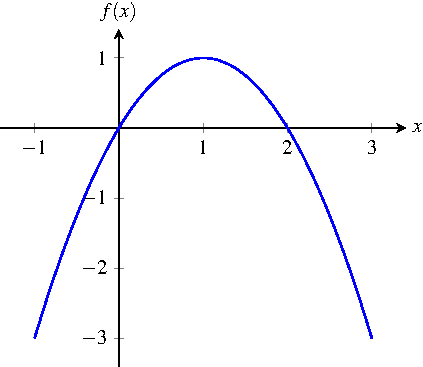
\includegraphics[scale=1.2]{image/09/largest-product.pdf}
\caption{%%
  A graph of the function $f(x) = -x^2 + 2x$.  The vertex of the
  function is the highest point in its graph.
}
\label{fig:largest_product_xy}
\end{figure}

From \Figure{fig:largest_product_xy}, you see that the largest value
of the product $xy = f(x)$ occurs at the vertex of $f(x)$.  The
horizontal coordinate of the vertex is
\[
x
=
-\frac{2}{2(-1)}
=
\frac{-2}{-2}
=
1.
\]
The vertical coordinate of the vertex is
\[
f(1)
=
-(1)^2 + 2(1)
=
-1 + 2
=
1.
\]
In other words, the largest value of the product $xy$ is $1$ and this
maximum value occurs when $x = 1$.

\solutionpart{subprob:maximum_product_given_sum_b}
You know that $x + y = b$.  Solve the last equation for $y$ to get
$y = b - x$ and you can now write the product $xy$ as the quadratic
function
\[
f(x)
=
x(b - x).
\]
Use the distributive laws to write the function $f(x)$ as
$f(x) = -x^2 + bx$.  You know that the vertex of $f(x)$ is the point
at which the value of $f(x)$ is highest or lowest.  The horizontal
coordinate of the vertex of $f(x)$ is
%%
\begin{align*}
x
&=
-\frac{b}{2(-1)} \\[4pt]
&=
\frac{b}{2}
\end{align*}
%%
so the corresponding vertical coordinate is
%%
\begin{align*}
f(b/2)
&=
\frac{b}{2} \parenthesis*{b - \frac{b}{2}} \\[4pt]
&=
\frac{b}{2} \parenthesis*{\frac{2b}{2} - \frac{b}{2}} \\[4pt]
&=
\frac{b}{2} \parenthesis*{\frac{b}{2}} \\[4pt]
&=
\frac{b^2}{4}.
\end{align*}
%%
Note that $f(b/2) = b^2 / 4$ is positive because you have assumed that
$b > 0$.  Therefore the quadratic function $f(x)$ has a maximum value
of $b^2 / 4$, which occurs when $x = b / 2$.

\solutionpart{subprob:minimum_product_given_difference_b}
You must express $y$ in terms of $x$ and $b$.  Solving the equation
$x - y = b$ for $y$ shows that you have $y = x - b$ and so the product
$xy$ can be written as the function
\[
f(x)
=
x(x - b).
\]
Use the distributive laws to expand the right-hand side and you can
write the latter expression as $f(x) = x^2 - bx$.  In the function
$f(x)$, you assume that you know the value of $b$~(i.e.~it is a
positive constant) and $x$ is the variable.  Since $f(x)$ represents
the product $xy$, the minimum or maximum value of $xy$ is equivalent
to the vertex of $f(x)$.  The horizontal coordinate of the vertex is
given by
%%
\begin{align*}
x
&=
-\frac{-b}{2(1)} \\[4pt]
&=
\frac{b}{2}.
\end{align*}
%%
The vertical coordinate of the vertex is
%%
\begin{align*}
f(b/2)
&=
\frac{b}{2}
\parenthesis*{\frac{b}{2} - b} \\[4pt]
&=
\frac{b}{2}
\parenthesis*{\frac{b}{2} - \frac{2b}{2}} \\[4pt]
&=
-\frac{b}{2} \cdot \frac{b}{2} \\[4pt]
&=
-\frac{b^2}{4}.
\end{align*}
%%
Therefore the least value of the product $xy$ is $-\frac{b^2}{4}$ and
this value occurs when $x = b/2$.
\end{solution}
}{}

\item A rectangle has a perimeter of $p > 0$.  Its length and width
  are $\ell$ and $w$, respectively.
  %%
  \begin{packedenum}
  \item\label{subprob:rectangle_length_w_p}
    Express the length in terms of the perimeter and width of the
    rectangle.

  \item\label{subprob:rectangle_maximum_area}
    Determine the maximum area of the rectangle.

  \item\label{subprob:rectangle_maximum_area_is_square}
    Show that the maximum area is obtained when the rectangle is a
    square.
  \end{packedenum}
\ifbool{showSolution}{
\begin{solution}
\solutionpart{subprob:rectangle_length_w_p}
You know that the perimeter is a positive number $p$.  Then the
perimeter can also be written as
\[
2w + 2\ell
=
p
\]
which factorises as $2(w + \ell) = p$.  Divide both sides by $2$ to
get $w + \ell = p / 2$ and solving for $\ell$ results in
$\ell = \frac{p}{2} - w$.

\solutionpart{subprob:rectangle_maximum_area}
The area of the rectangle can be written as $\ell w$.
Use \Part{subprob:rectangle_length_w_p} to write the area as
%%
\begin{align*}
f(w)
&=
w \parenthesis*{\frac{p}{2} - w} \\[4pt]
&=
-w^2 + \frac{p}{2}w.
\end{align*}
%%
The maximum area occurs at the vertex of $f(w)$.  The horizontal
coordinate of the vertex is
%%
\begin{align*}
w
&=
-\frac{p/2}{2(-1)} \\[4pt]
&=
\frac{p/2}{2} \\[4pt]
&=
\frac{p}{2} \times \frac{1}{2} \\[4pt]
&=
\frac{p}{4}.
\end{align*}
%%
The vertical coordinate of the vertex is
%%
\begin{align*}
f(p/4)
&=
\frac{p}{4}
\parenthesis*{
  \frac{p}{2} - \frac{p}{4}
} \\[4pt]
&=
\frac{p}{4}
\parenthesis*{
  \frac{2p}{4} - \frac{p}{4}
} \\[4pt]
&=
\frac{p}{4} \times \frac{p}{4} \\[4pt]
&=
\frac{p}{16}.
\end{align*}
%%
In other words, the maximum area of the rectangle is $p / 16$ and this
value occurs when the width is $w = p / 4$.

\solutionpart{subprob:rectangle_maximum_area_is_square}
From \Part{subprob:rectangle_length_w_p}, you know that the length can
be written as
%%
\begin{equation}
\label{eqn:rectangle_length_as_width_and_perimeter}
\ell
=
\frac{p}{2} - w.
\end{equation}
%%
From \Part{subprob:rectangle_maximum_area}, you know that the
rectangle attains its maximum area when its width is $w = p / 4$.
Substitute the latter expression in
\Equation{eqn:rectangle_length_as_width_and_perimeter} and you get
%%
\begin{align*}
\ell
&=
\frac{p}{2} - \frac{p}{4} \\[4pt]
&=
\frac{2p}{4} - \frac{p}{4} \\[4pt]
&=
\frac{p}{4}.
\end{align*}
%%
That is, when the area of the rectangle is maximised, the length and
width of the rectangle are the same.  Therefore given a perimeter
$p > 0$, the rectangle attains its maximum area when it is a square.
\end{solution}
}{}

\item\emph{FantasicTV.}
  Recall your work on regression with the data set for FantasicTV.
  Let $x$ be the selling price in dollars of each unit of FantasticTV.
  Let $S(x)$ be the number of units of FantasticTV sold at $x$ dollars
  each.  From your work on regression, you can approximate $S(x)$ as
  the linear function
  \[
  S(x)
  =
  90 - \frac{1}{10}x.
  \]
  Let $R(x)$ be a function for the \emph{revenue} in dollars.  The
  revenue is the amount of money you get from selling $S(x)$ units of
  FantasticTV at $x$ dollars each.  Note that the revenue is not the
  same as the profit you make from selling FantasticTV.  In order to
  calculate the profit, you must subtract the cost from the revenue.
  The cost includes money required for manufacturing and advertising
  your TVs.
  %%
  \begin{packedenum}
  \item\label{subprob:FantasticTV_total_revenue}
    Express the revenue as a quadratic function.

  \item\label{subprob:FantasticTV_zero_revenue_exist}
    Without calculating any specific selling prices, show that there
    is at least one selling price of each unit of FantasticTV such
    that the revenue is zero dollars.

  \item\label{subprob:FantasticTV_zero_revenue}
    Determine the selling prices of each unit of FantasticTV such that
    the revenue is zero dollars.

  \item\label{subprob:FantasticTV_maximize_revenue}
    Determine the selling price that would result in the maximum
    revenue.
  \end{packedenum}
\ifbool{showSolution}{
\begin{solution}
\solutionpart{subprob:FantasticTV_total_revenue}
The expression for revenue can be written as
%%
\begin{align*}
R(x)
&=
x \cdot S(x) \\[4pt]
&=
x \parenthesis*{90 - \frac{1}{10}x} \\[4pt]
&=
90x - \frac{1}{10}x^2.
\end{align*}

\solutionpart{subprob:FantasticTV_zero_revenue_exist}
The selling prices of each unit of FantasticTV such that the revenue
is zero dollars is equivalent to the roots of the quadratic function
$R(x)$.  Showing that such selling prices exist is equivalent to
showing that the discriminant of $R(x)$ is non-negative.  The
discriminant of $R(x)$ is given by
\[
\Delta
=
90^2 - 4\parenthesis*{-\frac{1}{10}}(0)
=
90^2
\]
which is positive.  Therefore there are two different selling prices
such that the revenue is zero dollars.

\solutionpart{subprob:FantasticTV_zero_revenue}
The selling prices of each unit of FantasticTV such that the revenue
is zero dollars is equivalent to the roots of the quadratic function
$R(x)$.  The quadratic formula shows that the roots of $R(x)$ are
given by
%%
\begin{align*}
x
&=
\frac{
  -90 \pm \sqrt{\Delta}
}{
  2\parenthesis*{-\frac{1}{10}}
} \\[4pt]
&=
\frac{
  -90 \pm \sqrt{90^2}
}{
  2\parenthesis*{-\frac{1}{10}}
} \\[4pt]
&=
\frac{
  -90 \pm 90
}{
  -\frac{1}{5}
}.
\end{align*}
%%
The specific selling prices that would result in zero revenue are
$x = 0$ dollars and $x = 900$ dollars.

\solutionpart{subprob:FantasticTV_maximize_revenue}
The selling price that would result in the highest revenue is
equivalent to the vertex of the function $R(x)$.  The horizontal
coordinate of the vertex is
\[
x
=
-\frac{
  90
}{
  2\parenthesis*{-\frac{1}{10}}
}
=
450
\]
and the vertical coordinate of the vertex is
\[
R(450)
=
90(450) - \frac{450^2}{10}
=
20,250.
\]
Therefore if each unit of FantasticTV is sold at $450$ dollars, then
the maximum revenue would be $20,250$ dollars.
\end{solution}
}{}

\item A cannon is buried underground such that the tip of the cannon
  is at ground level.  The canon fires a cannonball whose path through
  the air is described by the function $f(x) = bx - x^2$.  Here $x$ is
  the horizontal distance between the cannonball and the tip of the
  cannon, $f(x)$ is the vertical distance from the cannonball to the
  ground, and $b > 0$ is a constant.  Next to the cannon is a toy
  rocket that is tilted at $\degree{45}$ with respect to ground level.
  When the rocket is launched, it travels in a straight line whose
  path is described by the function $g(x) = x$.  Here $x$ is the
  horizontal distance between the rocket and its launch site and
  $g(x)$ represents the vertical distance between the rocket and
  ground level.  Suppose that all distances are measured in metres.
  Further suppose that the rocket is launched at the same time as when
  the cannonball is fired.  You may assume that the rocket has enough
  fuel to propel itself even after the cannonball has reached the
  ground.  Determine the horizontal distances at which both the rocket
  and the cannonball are the same vertical distance from ground
  level.
\ifbool{showSolution}{
\begin{solution}
\Figure{fig:path_cannonball_rocket} shows a rough sketch of the paths
of the cannonball and rocket.  The figure shows two points of
intersection between the functions $f(x)$ and $g(x)$.  Each point of
intersection represents the horizontal distance at which both the
cannonball and the rocket are at the same distance from ground level.

\begin{figure}[!htbp]
\centering
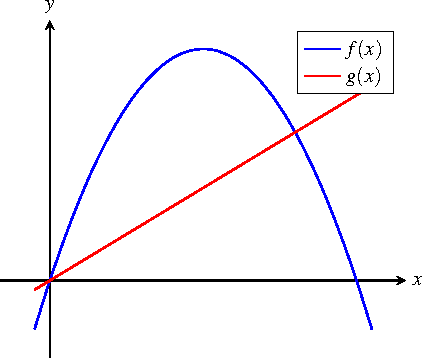
\includegraphics[scale=1.2]{image/09/rocket-cannonball.pdf}
\caption{%%
  The paths of two projectiles on one set of coordinate axes.  The
  blue graph represents the path of the cannonball.  The red graph
  represents the path of the rocket.  The variable $x$ represents the
  horizontal distance between the projectile and the site from where
  it was launched.  The function value~(i.e.~$f(x)$ or $g(x)$)
  represents the vertical distance from the projectile to ground
  level.
}
\label{fig:path_cannonball_rocket}
\end{figure}

To calculate the points of intersection, you equate the two functions
and solve for $x$.  Equating the two functions shows that you have
$f(x) = g(x)$, which can also be written as
\[
bx - x^2
=
x.
\]
Moving everything to the left-hand side results in
$-x^2 + bx - x = 0$.  In the latter expression, you can factorise $x$
to get
%%
\begin{equation}
\label{eqn:quadratic_point_of_intersection}
(b - 1 - x)x
=
0.
\end{equation}
%%
If you define the function $h(x) = (b - 1 - x)x$, then
\Expression{eqn:quadratic_point_of_intersection} can be written more
compactly as $h(x) = 0$, which says that you want to determine all
roots of $h(x)$.  As $h(x)$ is a quadratic function, you can use the
quadratic formula to determine the roots.

On the other hand, you can also determine the roots of $h(x)$ without
using the quadratic formula.  This requires some close observation of
$h(x)$.  Carefully note what
\Expression{eqn:quadratic_point_of_intersection} is telling you.  In
general, the expression says that when you multiply two numbers
together you get zero.  If that is the case, then one~(or both) of
those two numbers must be zero.  In
\Expression{eqn:quadratic_point_of_intersection}, your two numbers are
$x$ and $b - 1 - x$.  Which values of $x$ would make
\Expression{eqn:quadratic_point_of_intersection} true?  If $x = 0$,
then \Expression{eqn:quadratic_point_of_intersection} would certainly
be true.  If $b - 1 - x = 0$, then
\Expression{eqn:quadratic_point_of_intersection} would also be true.
Solving $b - 1 - x = 0$ for $x$ yields $x = b - 1$.  In other words,
one point of intersection is at $x = 0$ and the corresponding function
value is
\[
f(0)
=
0
=
g(0).
\]
This tells you that when the cannonball and rocket are both on the
ground, then they are at the same vertical distance~(which is zero
metres) from ground level.  The other point of intersection occurs at
$x = b - 1$ with the corresponding function value being
%%
\begin{align*}
f(b - 1)
&=
(b - 1)\bigparen{b - (b - 1)} \\[4pt]
&=
(b - 1) (b - b + 1) \\[4pt]
&=
b - 1 \\[4pt]
&=
g(b - 1).
\end{align*}
%%
This tells you that when the cannonball and rocket are at a horizontal
distance of $b - 1$ metres from their site of launch, then they are
both at a vertical distance of $b - 1$ metres from ground level.
\end{solution}
}{}

\begin{table}[!htbp]
\centering
\begin{tabular}{lrrrr}                                                 \toprule
        & Distance to & \multicolumn{3}{c}{Orbital period~(Earth days)} \\
  \cmidrule{3-5}
Planet  & Sun~(Gm)    & Observed  & Kepler & Quadratic \\\midrule
Mercury & $57.9$                  & $88.0$     \\[4pt]
Venus   & $108.2$                 & $224.7$    \\[4pt]
Earth   & $149.6$                 & $365.2$    \\[4pt]
Mars    & $227.9$                 & $687.0$    \\[4pt]
Jupiter & $778.6$                 & $4331.0$   \\[4pt]
Saturn  & $1433.5$                & $10,747.0$ \\[4pt]
Uranus  & $2872.5$                & $30,589.0$ \\[4pt]
Neptune & $4495.4$                & $59,800.0$ \\[4pt]
Pluto   & $5906.4$                & $90,560.0$ \\\bottomrule
\end{tabular}

\caption{%%
  The orbital period of a planet as a function of its distance~(in
  gigametres) to the Sun.  The third, fourth, and fifth columns are
  reserved for the orbital periods~(observed, Kepler's equation,
  quadratic equation) of each planet.  The orbital period of a planet
  is the number of Earth days required for the planet to complete one
  orbit around the Sun.  The planet Earth has an orbital period of
  $365.2$ Earth days.  The third column contains the observed orbital
  period of each planet, as provided by NASA.  The fourth column
  should contain the orbital periods as calculated by Kepler's
  \Equation{eqn:Earth_days_orbit_Kepler}.  The fifth column should
  contain the orbital periods as calculated by the quadratic
  \Equation{eqn:Earth_days_orbit_approximation}.
}
\label{tab:planet_distance_to_Sun}
\end{table}

\item\emph{Orbital period.}
  In the Solar System, the distance from any planet to the Sun is
  measured in terms of astronomical unit~(in symbol AU).  One
  astronomical unit~(or $1$~AU) is defined by the International
  Astronomical Union as equivalent to exactly $149,597,870,700$
  metres,\footnote{
    See the following document for further details:
    \url{http://web.archive.org/web/20180427004114/https://www.iau.org/static/resolutions/IAU2012_English.pdf},
    accessed 2018-04-27.
  }
  which is roughly the average distance from Earth to the Sun.
  Dividing one astronomical unit by $1000$ gives
  %%
  \begin{equation}
  \label{eqn:astronomical_unit_over_1000}
  149597870700 / 1000
  =
  149,597,870.7
  \end{equation}
  %%
  kilometres.  You can also measure the distance from any planet to
  the Sun in terms of gigametres~(or Gm).  One gigametre~(or $1$~Gm)
  is equivalent to $10^6$ kilometres.  Dividing
  \Expression{eqn:astronomical_unit_over_1000} by $10^6$ shows that
  one astronomical unit is equivalent to
  \[
  149597870.7 / 10^6
  =
  149.5978707
  \]
  gigametres.  In other words, the average distance from Earth to the
  Sun is approximately $149.6$ Gm, rounded to one decimal place.
  Suppose $x$ represents the distance~(in gigametres) from a planet to
  the Sun.  If $f(x)$ represents the number of Earth days required for
  a planet to complete one orbit around the sun, then $f(x)$ can be
  approximated as the quadratic function
  %%
  \begin{equation}
  \label{eqn:Earth_days_orbit_approximation}
  f(x)
  =
  0.0016x^2 + 6.3044x - 770.2297.
  \end{equation}
  %%
  \begin{packedenum}
  \item\label{subprob:planetary_orbit_quadratic}
    \Table{tab:planet_distance_to_Sun} shows the distances~(in Gm) of
    various planets to the Sun and the corresponding orbital periods.
    The data are provided by NASA.\footnote{
      See the following website:
      \url{http://web.archive.org/web/20180427010804/https://nssdc.gsfc.nasa.gov/planetary/factsheet/},
      accessed 2018-04-27.
    }
    Use \Expression{eqn:Earth_days_orbit_approximation} to fill in the
    missing entries of column $5$ of
    \Table{tab:planet_distance_to_Sun}.

  \item\label{subprob:planetary_orbit_Kepler}
    In the $17$-th century, Johannes Kepler discovered a formula to
    determine the orbital period of planets in the Solar System.
    Kepler found that if $x$ represents the distance~(in gigametres)
    from a planet to the Sun, then the number $g(x)$ of Earth days
    required for the planet to complete one orbit around the Sun is
    given by\footnote{
      The equation is from page~27 of the following book:
      \url{http://web.archive.org/web/20180427045920/https://www.eoas.ubc.ca/books/Practical_Meteorology/prmet102/Practical_Meteorology-v1.02b-WholeBookColor.pdf},
      accessed 2018-04-27.
    }
    %%
    \begin{equation}
    \label{eqn:Earth_days_orbit_Kepler}
    g(x)
    =
    0.1996x^{1.5}.
    \end{equation}
    %%
    Use \Equation{eqn:Earth_days_orbit_Kepler} to fill in the missing
    entries of column $4$ of \Table{tab:planet_distance_to_Sun}.

  \item\label{subprob:planetary_orbit_comparison}
    You now have two
    functions~(i.e.~\Equations{eqn:Earth_days_orbit_approximation}{eqn:Earth_days_orbit_Kepler})
    that model the orbital period of a planet given the distance of
    the planet from the Sun.  How do you decide which of the two
    functions is better?  One way to help you decide is to graph the
    \emph{errors} of each function.  Here, the word \emph{error}
    means: how far away is the predicted value from the observed
    value.  In this case, observed values are listed in the
    ``Observed'' column of \Table{tab:planet_distance_to_Sun}.  A
    predicted value is a value of the orbital period as calculated by
    some function.  Let $\tuple{d}{p}$ be a data point from
    \Table{tab:planet_distance_to_Sun}, where $d$ denotes the
    distance~(in Gm) from a planet to the Sun and $p$ represents the
    orbital period~(in Earth days) of the planet.  The observed
    orbital period is $p$.  The orbital periods as predicted by
    \Equations{eqn:Earth_days_orbit_approximation}{eqn:Earth_days_orbit_Kepler}
    are, respectively, $f(d)$ and $g(d)$.  The error of $f(x)$ at
    $x = d$ is $f(d) - p$ and the error of $g(x)$ at $x = d$ is
    $g(d) - p$.  Then the errors of the functions $f(x)$ and $g(x)$
    are, respectively, the errors $f(d) - p$ and $g(d) - p$ for each
    data point $\tuple{d}{p}$.  Add another two columns to
    \Table{tab:planet_distance_to_Sun}.  One column should list the
    errors of $f(x)$ and the other column the errors of $g(x)$.  Graph
    the distances versus the errors of $f(x)$.  On the same set of
    axes, graph the distances versus the errors of $g(x)$.  What do
    you notice when an error is negative?  How would you interpret a
    positive error?

  \item\label{subprob:planetary_orbit_RMS_error}
    You can use the \emph{root mean square error}~(or RMS error) to
    help you decide which function is better than the other at
    modelling the observed orbital periods.  The better is a function
    at modelling the orbital periods given in
    \Table{tab:planet_distance_to_Sun}, the lower should be its RMS
    error.  Let $y_i$ be the observed~(i.e.~exact) orbital period of
    planet $i$ and suppose that $\widehat{y_i}$ is the predicted
    orbital period of planet $i$ as calculated by some function.  If
    you have $n$ observed values $\seq{y_1}{y_2}{y_n}$ and $n$
    predicted values
    $\seq{\widehat{y_1}}{\widehat{y_2}}{\widehat{y_n}}$, then the
    error of the $i$-th predicted value is given by
    $\widehat{y_i} - y_i$, which means ``prediction minus observed''.
    Then the squared error is $(\widehat{y_i} - y_i)^2$.  Calculate
    the mean of all the squared errors and take the square root of the
    mean.  The result is the RMS error, which can be written as the
    expression
    %%
    \begin{align*}
    \text{RMS error}
    &=
    \sqrt{
      \frac{1}{n}
      \sum_{i=1}^n (\widehat{y_i} - y_i)^2
    } \\[4pt]
    &=
    \sqrt{
      \frac{
        \sumseq{
          (\widehat{y_1} - y_1)^2
        }{
          (\widehat{y_2} - y_2)^2
        }{
          (\widehat{y_n} - y_n)^2
        }
      }{
        n
      }
    }.
    \end{align*}
    %%
    Use the RMS errors to help you explain which one of
    \Equations{eqn:Earth_days_orbit_approximation}{eqn:Earth_days_orbit_Kepler}
    is better than the other at modelling the orbital periods of the
    planets listed in \Table{tab:planet_distance_to_Sun}.
  \end{packedenum}
\ifbool{showSolution}{
\begin{solution}
\solutionpart{subprob:planetary_orbit_quadratic}
\solutionpart{subprob:planetary_orbit_Kepler}
\solutionpart{subprob:planetary_orbit_comparison}
\Table{tab:planet_orbital_periods_errors} shows the completed version
of \Table{tab:planet_distance_to_Sun} with all missing entries filled
in.  The table also shows the errors of the functions $f(x)$ and
$g(x)$.  The errors are graphed in
\Figure{fig:orbital_periods_error_analysis}.  Let $\tuple{d}{p}$ be a
data point from \Table{tab:planet_distance_to_Sun}, where $d$ is the
distance~(in Gm) from a planet to the Sun and $p$ is the orbital
period of the planet.  If the error $f(d) - p$ is negative, then the
predicted orbital period $f(d)$ underestimates the observed orbital
period $p$.  On the other hand, if the error $f(d) - p$ is positive,
the predicted orbital period $f(d)$ overestimates the observed orbital
period $p$.  A similar comment applies to the function $g(x)$.  In
terms of the error graphs in
\Figure{fig:orbital_periods_error_analysis}, if part of an error graph
is above the horizontal axis~(the horizontal line through the origin)
then that part overestimates the observed orbital periods.  Similarly,
if a part of the error graph is below the horizontal exis, then that
part of the graph underestimates the observed orbital periods.  The
closer is an error graph to the horizontal axis, the better is the
corresponding function at predicting the orbital periods.

\begin{table}[!htbp]
\centering
\begin{tabular}{lrrrrrrr} \toprule
        & Distance to & \multicolumn{3}{c}{Orbital period~(Earth days)} && \multicolumn{2}{c}{Error} \\
  \cmidrule{3-5} \cmidrule{7-8}
Planet  & Sun~(Gm)    & Observed     & Kepler    & Quadratic && Kepler   & Quadratic \\\midrule
Mercury & $57.9$      & $88.0$       & $87.9$    & $-399.8$  && $-0.06$  & $-487.84$ \\
Venus   & $108.2$     & $224.7$      & $224.6$   & $-69.4$   && $-0.05$  & $-294.06$ \\
Earth   & $149.6$     & $365.2$      & $365.2$   & $208.7$   && $0.02$   & $-156.48$ \\
Mars    & $227.9$     & $687.0$      & $686.7$   & $749.6$   && $-0.28$  & $62.64$   \\
Jupiter & $778.6$     & $4331.0$     & $4336.4$  & $5108.3$  && $5.43$   & $777.32$  \\
Saturn  & $1433.5$    & $10747.0$    & $10833.2$ & $11555.0$ && $86.21$  & $808.00$  \\
Uranus  & $2872.5$    & $30589.0$    & $30729.2$ & $30541.2$ && $140.15$ & $-47.83$  \\
Neptune & $4495.4$    & $59800.0$    & $60160.7$ & $59904.4$ && $360.72$ & $104.36$  \\
Pluto   & $5906.4$    & $90560.0$    & $90603.5$ & $92283.0$ && $43.47$  & $1722.98$ \\\bottomrule
\end{tabular}

\caption{%%
  The orbital period of a planet as a function of its distance~(in
  gigametres) to the Sun.  This is the same as
  \Table{tab:planet_distance_to_Sun}, but missing entries have been
  filled in.  All numbers in the fourth and fifth columns have been
  rounded to one decimal place.  The sixth and seventh columns list,
  respectively, the errors of Kepler's
  \Equation{eqn:Earth_days_orbit_Kepler} and the quadratic
  \Equation{eqn:Earth_days_orbit_approximation}.  Numbers in these
  columns have been rounded to two decimal places.  Note that most
  numbers in the table have been rounded in order to fit the table.
  However, you should not round these intermediate results when you
  use them to calculate the root mean square errors.
}
\label{tab:planet_orbital_periods_errors}
\end{table}

\begin{figure}[!htbp]
\centering
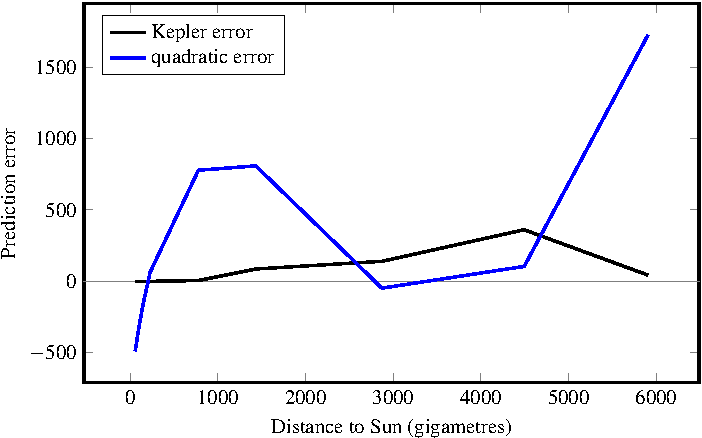
\includegraphics[scale=1.1]{image/09/period-error.pdf}
\caption{%%
  The errors of Kepler's function~\eqref{eqn:Earth_days_orbit_Kepler}
  and the quadratic
  function~\eqref{eqn:Earth_days_orbit_approximation}.
}
\label{fig:orbital_periods_error_analysis}
\end{figure}

\solutionpart{subprob:planetary_orbit_RMS_error}
The RMS error of Kepler's \Equation{eqn:Earth_days_orbit_Kepler} is
$132.9641$, which is smaller than the RMS error of $714.2830$ of the
quadratic \Equation{eqn:Earth_days_orbit_approximation}, both numbers
rounded to four decimal places.  Therefore you may conclude that
Kepler's equation provides a better model of the orbital periods of
the given planets than does the quadratic function.
\end{solution}
}{}

\item\emph{Quadratic regression.}
  Recall that linear regression allows you to determine a linear
  function that best fits a given data set.  In this problem, you will
  learn another technique called \emph{quadratic regression} that
  allows you to determine a quadratic function that best fits a given
  data set.  Quadratic regression requires a mathematical object
  called \emph{matrices}.
  %%
  \begin{packedenum}
  \item\label{subprob:quadratic_applications:matrix_sum}
    A $2 \times 2$ matrix is an array that has $2$ rows and $2$
    columns.  A $3 \times 3$ matrix is an array having $3$ rows and
    $3$ columns.  In general, an $n \times m$ matrix is an array
    containing $n$ rows and $m$ columns.  The following are examples
    of matrices:
    \[
    \begin{bmatrix}
    1 & 2 \\
    3 & 4
    \end{bmatrix},
    %%
    \qquad
    %%
    \begin{bmatrix}
    1 & 2 & 3 \\
    4 & 5 & 6 \\
    7 & 8 & 9
    \end{bmatrix},
    %%
    \qquad
    %%
    \begin{bmatrix}
    3 & 5 & 4 \\
    1 & 9 & 2
    \end{bmatrix}.
    \]
    Going from left to right, you have a $2 \times 2$ matrix, a
    $3 \times 3$ matrix, and a $2 \times 3$ matrix.  Let $\matA$ and
    $\matB$ be $2 \times 2$ matrices defined by
    %%
    \begin{equation}
    \label{eqn:quadratic_applications:2x2_matrices}
    \matA
    =
    \begin{bmatrix}
    a & b \\
    c & d
    \end{bmatrix}
    %%
    \qquad
    \text{and}
    \qquad
    %%
    \matB
    =
    \begin{bmatrix}
    e & f \\
    g & h
    \end{bmatrix}
    \end{equation}
    %%
    where $\octuple{a}{b}{c}{d}{e}{f}{g}{h}$ are any real numbers.
    You add the matrices by adding the corresponding elements.  Thus
    the matrix sum $\matA + \matB$ is defined as
    \[
    \matA + \matB
    =
    \begin{bmatrix}
    a + e & b + f \\
    c + g & d + h
    \end{bmatrix}.
    \]
    Similarly, if $\matC$ and $\matD$ are $3 \times 3$ matrices
    defined by
    %%
    \begin{equation}
    \label{eqn:quadratic_applications:3x3_matrices}
    \matC
    =
    \begin{bmatrix}
    a_1 & b_1 & c_1 \\
    a_2 & b_2 & c_2 \\
    a_3 & b_3 & c_3
    \end{bmatrix}
    %%
    \qquad
    \text{and}
    \qquad
    %%
    \matD
    =
    \begin{bmatrix}
    d_1 & e_1 & f_1 \\
    d_2 & e_2 & f_2 \\
    d_3 & e_3 & f_3
    \end{bmatrix}
    \end{equation}
    %%
    where the $\sextuple{a_i}{b_i}{c_i}{d_i}{e_i}{f_i}$ are any real
    numbers, then the matrix sum $\matC + \matD$ is defined as
    \[
    \matC + \matD
    =
    \begin{bmatrix}
    a_1 + d_1 & b_1 + e_1 & c_1 + f_1 \\
    a_2 + d_2 & b_2 + e_2 & c_2 + f_2 \\
    a_3 + d_3 & b_3 + e_3 & c_3 + f_3
    \end{bmatrix}.
    \]
    Two matrices must have the same number of rows and columns in
    order that they can be added together.\footnote{
      See also the website
      \url{http://web.archive.org/web/20180529163624/https://www.mathsisfun.com/algebra/matrix-introduction.html},
      accessed 2018-05-29 and the video at
      \url{https://youtu.be/WR9qCSXJlyY}.
    }
    Consider the matrices
    %%
    \begin{equation}
    \label{eqn:quadratic_applications:matrices_for_sum_product}
    \begin{aligned}
    \matE
    =
    \begin{bmatrix}
    2 & 3 \\
    5 & 7
    \end{bmatrix},
    %%
    &\qquad
    %%
    \matF
    =
    \begin{bmatrix}
    1 & 4 \\
    6 & 8
    \end{bmatrix}, \\[4pt]
    %%
    \matG
    =
    \begin{bmatrix}
    10 & 3  & 5  \\
    7  & 9  & 11 \\
    13 & 15 & 17
    \end{bmatrix},
    %%
    &\qquad
    \matH
    =
    \begin{bmatrix}
    4 & 13 & 2  \\
    6 & 9  & 10 \\
    8 & 5  & 3
    \end{bmatrix}.
    \end{aligned}
    \end{equation}
    %%
    Calculate the matrix sums $\matE + \matF$, $\matG + \matH$, and
    $\matE + \matG$.

  \item\label{subprob:quadratic_applications:matrix_product}
    You can also multiply matrices, but there are restrictions on
    which matrices can be multiplied by which other matrices.  The
    usual matrix product is called the \emph{dot product}.  If you
    have an $m \times n$ matrix $\alpha$ and an $n \times p$ matrix
    $\beta$, then you can perform the dot product
    $\alpha \times \beta = \alpha\beta$ because the number of columns
    in $\alpha$ is the same as the number of rows in $\beta$.  The dot
    product $\alpha\beta$ is an $m \times p$ matrix.\footnote{
      See also the website
      \url{http://web.archive.org/web/20180529165826/https://www.mathsisfun.com/algebra/matrix-multiplying.html},
      accessed 2018-05-29 and the video at
      \url{https://youtu.be/OMA2Mwo0aZg}.
    }
    Given the $2 \times 2$ matrices $\matA$ and $\matB$ as defined
    in~\eqref{eqn:quadratic_applications:2x2_matrices}, the dot
    product $\matA \matB$ is defined as
    \[
    \matA \matB
    =
    \begin{bmatrix}
    ae + bg & af + bh \\
    ce + dg & cf + dh
    \end{bmatrix}.
    \]
    Given the $3 \times 3$ matrices $\matC$ and $\matD$ as defined
    in~\eqref{eqn:quadratic_applications:3x3_matrices}, the dot
    product $\matC \matD$ is defined by
    \[
    \matC \matD
    =
    \begin{bmatrix}
    a_1d_1 + b_1d_2 + c_1d_3 & a_1e_1 + b_1e_2 + c_1e_3 & a_1f_1 + b_1f_2 + c_1f_3 \\
    a_2d_1 + b_2d_2 + c_2d_3 & a_2e_1 + b_2e_2 + c_2e_3 & a_2f_1 + b_2f_2 + c_2f_3 \\
    a_3d_1 + b_3d_2 + c_3d_3 & a_3e_1 + b_3e_2 + c_3e_3 & a_3f_1 + b_3f_2 + c_3f_3
    \end{bmatrix}.
    \]
    Let $\quadruple{\matE}{\matF}{\matG}{\matH}$ be matrices as
    defined
    in~\eqref{eqn:quadratic_applications:matrices_for_sum_product}.
    Calculate the dot products $\matE \matF$, $\matF \matE$,
    $\matG \matH$, and $\matE \matG$.

  \item\label{subprob:quadratic_applications:matrix_determinant}
    Matrices have an operation called the \emph{determinant}, which is
    defined only for any matrix whose number of rows is the same as
    its number of columns.\footnote{
      See the website
      \url{http://web.archive.org/web/20180529190146/https://www.mathsisfun.com/algebra/matrix-determinant.html},
      accessed 2018-05-29 and the video at
      \url{https://youtu.be/0c7dt2SQfLw}.
    }
    Consider the $2 \times 2$ matrix $\matA$ as defined
    in~\eqref{eqn:quadratic_applications:2x2_matrices}.  The
    determinant of $\matA$ is written as $\det(\matA)$ and is defined
    as
    %%
    \begin{align*}
    \det(\matA)
    &=
    \begin{vmatrix}
    a & b \\
    c & d
    \end{vmatrix} \\[4pt]
    &=
    ad - bc.
    \end{align*}
    %%
    The determinant of a $3 \times 3$ matrix can be defined in terms
    of the determinant of $2 \times 2$ matrices.  Consider the
    $3 \times 3$ matrix $\matC$ as defined
    in~\eqref{eqn:quadratic_applications:3x3_matrices}.  The
    determinant of $\matC$ is defined as
    %%
    \begin{align*}
    \det(\matC)
    &=
    \begin{vmatrix}
    a_1 & b_1 & c_1 \\
    a_2 & b_2 & c_2 \\
    a_3 & b_3 & c_3
    \end{vmatrix} \\[4pt]
    &=
    a_1
    \begin{vmatrix}
    b_2 & c_2 \\
    b_3 & c_3
    \end{vmatrix}
    -
    b_1
    \begin{vmatrix}
    a_2 & c_2 \\
    a_3 & c_3
    \end{vmatrix}
    +
    c_1
    \begin{vmatrix}
    a_2 & b_2 \\
    a_3 & b_3
    \end{vmatrix}.
    \end{align*}
    %%
    Calculate the determinant of each matrix
    in~\eqref{eqn:quadratic_applications:matrices_for_sum_product}.

  \item\label{subprob:quadratic_applications:bluegill_data}
    The file \code{bluegill.csv} contains data on the age and length
    of $78$ bluegill sunfish that were sampled from Lake Mary,
    Minnesota, USA during June of~1981.\footnote{
      The data set is due to Richard V. Frie in the paper
      \url{https://doi.org/10.1577/1548-8446(1982)007<0005:MOFSAB>2.0.CO;2},
      but the full data set was published in the paper
      \url{https://doi.org/10.1080/01621459.1986.10478351}.
    }
    The age of a bluegill sunfish is the measured age~(in years) at
    the time the fish was captured and the length of the fish is
    measured in millimetres.  Produce a scatter plot of the age versus
    length of the bluegill sunfish.  Explain what you notice about the
    graph.

  \item\label{subprob:quadratic_applications:bluegill_regression}
    For the data set \code{bluegill.csv}, let $x$ and $y$ denote the
    age and length, respectively.  Then $x_i$ denotes the $i$-th row
    in the age column and $y_i$ represents the $i$-th row in the
    length column.  Let $f(x)$ be the length~(mm) of a bluegill
    sunfish whose age at capture is $x$ years.  Assuming that the data
    set can be modelled as a quadratic function, then $f(x)$ can be
    written as $f(x) = ax^2 + bx + c$ with $a \neq 0$.  Here, the
    parameters $\triple{a}{b}{c}$ must be estimated by using the given
    data.  The parameters and the data can be written as the matrix
    equation
    %%
    \begin{equation}
    \label{eqn:quadratic_applications:bluegill_matrix_equation}
    \begin{bmatrix}
    \sum_{i=1}^n x_i^4 & \sum_{i=1}^n x_i^3 & \sum_{i=1}^n x_i^2 \\[4pt]
    \sum_{i=1}^n x_i^3 & \sum_{i=1}^n x_i^2 & \sum_{i=1}^n x_i   \\[4pt]
    \sum_{i=1}^n x_i^2 & \sum_{i=1}^n x_i   & n
    \end{bmatrix}
    %%
    \begin{bmatrix}
    a \\[4pt]
    b \\[4pt]
    c
    \end{bmatrix}
    =
    \begin{bmatrix}
    \sum_{i=1}^n x_i^2 y_i \\[4pt]
    \sum_{i=1}^n x_i y_i \\[4pt]
    \sum_{i=1}^n y_i
    \end{bmatrix}
    \end{equation}
    %%
    where $n = 78$ is the number of data points.  You can use a
    technique called \emph{Cramer's rule} to determine the values of
    the parameters $\triple{a}{b}{c}$.  Define the determinants
    %%
    \begin{align*}
    &D
    =
    \begin{vmatrix}
    \sum_{i=1}^n x_i^4 & \sum_{i=1}^n x_i^3 & \sum_{i=1}^n x_i^2 \\[4pt]
    \sum_{i=1}^n x_i^3 & \sum_{i=1}^n x_i^2 & \sum_{i=1}^n x_i   \\[4pt]
    \sum_{i=1}^n x_i^2 & \sum_{i=1}^n x_i   & n
    \end{vmatrix},
    %%
    \quad
    %%
    D_a
    =
    \begin{vmatrix}
    \sum_{i=1}^n x_i^2y_i & \sum_{i=1}^n x_i^3 & \sum_{i=1}^n x_i^2 \\[4pt]
    \sum_{i=1}^n x_iy_i   & \sum_{i=1}^n x_i^2 & \sum_{i=1}^n x_i   \\[4pt]
    \sum_{i=1}^n y_i      & \sum_{i=1}^n x_i   & n
    \end{vmatrix}, \\[4pt]
    %%
    &D_b
    =
    \begin{vmatrix}
    \sum_{i=1}^n x_i^4 & \sum_{i=1}^n x_i^2y_i & \sum_{i=1}^n x_i^2 \\[4pt]
    \sum_{i=1}^n x_i^3 & \sum_{i=1}^n x_iy_i   & \sum_{i=1}^n x_i   \\[4pt]
    \sum_{i=1}^n x_i^2 & \sum_{i=1}^n y_i      & n
    \end{vmatrix},
    %%
    \quad
    %%
    D_c
    =
    \begin{vmatrix}
    \sum_{i=1}^n x_i^4 & \sum_{i=1}^n x_i^3 & \sum_{i=1}^n x_i^2y_i \\[4pt]
    \sum_{i=1}^n x_i^3 & \sum_{i=1}^n x_i^2 & \sum_{i=1}^n x_iy_i   \\[4pt]
    \sum_{i=1}^n x_i^2 & \sum_{i=1}^n x_i   & y_i
    \end{vmatrix}.
    \end{align*}
    %%
    Cramer's rule states that the values of $\triple{a}{b}{c}$ in
    \Equation{eqn:quadratic_applications:bluegill_matrix_equation} can
    be written as
    \[
    a
    =
    \frac{D_a}{D},
    %%
    \qquad
    %%
    b
    =
    \frac{D_b}{D},
    %%
    \qquad
    %%
    c
    =
    \frac{D_c}{D}
    \]
    provided that the determinant $D \neq 0$.  Use the given data set
    to estimate the values of $\triple{a}{b}{c}$ in the function
    $f(x) = ax^2 + bx + c$.  Graph your formula together with the
    scatter plot
    from \Part{subprob:quadratic_applications:bluegill_data}.

  \item\label{subprob:quadratic_applications:bluegill_coefficient_determination}
    Given a regression function of a data set, the
    \emph{coefficient of determination} is a number that measures how
    well the regression function fits the data.  This is similar to
    the way the Pearson correlation coefficient measures how well a
    linear regression function fits a data set.  The coefficient of
    determination is denoted by $R^2$ and is always between $0$ and
    $1$, inclusive.  The closer is $R^2$ to $1$, the better is the fit
    of a regression function to the given data.  The value of $R^2$
    for linear regression is calculated by squaring the Pearson
    correlation coefficient.  In the case of quadratic regression, the
    value of $R^2$ is defined as follows.  Given a data point
    $\tuple{x_i}{y_i}$ and a quadratic regression function
    $f(x) = ax^2 + bx + c$, the error of $f(x)$ at the point
    $\tuple{x_i}{y_i}$ is defined as the difference between $f(x_i)$
    and $y_i$.  The error of $f(x)$ at $\tuple{x_i}{y_i}$ can be
    written as $y_i - f(x_i) = y_i - ax_i^2 - bx_i - c$.  The sum of
    the squared errors~(SSE) is written as
    \[
    \text{SSE}
    =
    \sum_{i=1}^n (y_i - ax_i^2 - bx_i - c)^2
    \]
    where $n$ denotes the number of data points.  If $\ybar$ is the
    mean of the $y_i$, the total sum of squares~(TSS) is defined as
    \[
    \text{TSS}
    =
    \sum_{i=1}^n (y_i - \ybar)^2.
    \]
    The SSE and TSS can be used to write the coefficient of
    determination of $f(x)$ as
    \[
    R^2
    =
    1
    -
    \frac{\text{SSE}}{\text{TSS}}
    =
    1
    -
    \frac{
      \sum_{i=1}^n (y_i - ax_i^2 - bx_i - c)^2
    }{
      \sum_{i=1}^n (y_i - \ybar)^2
    }.
    \]
    Calculate the coefficient of determination of your quadratic
    regression function
    from \Part{subprob:quadratic_applications:bluegill_regression}.

  \item\label{subprob:quadratic_applications:bluegill_linear_regression}
    Suppose that the data in the file \code{bluegill.csv} can be
    modelled as a linear function $g(x)$.  Use linear regression on
    the data set to estimate the parameters of $g(x)$.  Plot the
    function $g(x)$ together with the graph
    from \Part{subprob:quadratic_applications:bluegill_regression}.
    Calculate the coefficient of determination of $g(x)$.  Use the
    values of $R^2$ and the root mean square errors for $f(x)$ and
    $g(x)$ to help you decide which one of the two functions is better
    than the other at modelling the given data set.
  \end{packedenum}
\ifbool{showSolution}{
\begin{solution}
\solutionpart{subprob:quadratic_applications:matrix_sum}
The matrices $\matE$ and $\matF$ as defined
in~\eqref{eqn:quadratic_applications:matrices_for_sum_product} have
the sum
%%
\begin{align*}
\matE + \matF
&=
\begin{bmatrix}
2 & 3 \\
5 & 7
\end{bmatrix}
+
\begin{bmatrix}
1 & 4 \\
6 & 8
\end{bmatrix} \\[4pt]
&=
\begin{bmatrix}
2 + 1 & 3 + 4 \\
5 + 6 & 7 + 8
\end{bmatrix} \\[4pt]
&=
\begin{bmatrix}
3 & 7 \\
11 & 15
\end{bmatrix}.
\end{align*}
%%
Similarly, the matrices $\matG$ and $\matH$ as defined
in~\eqref{eqn:quadratic_applications:matrices_for_sum_product} have
the sum
%%
\begin{align*}
\matG + \matH
&=
\begin{bmatrix}
10 & 3  & 5  \\
7  & 9  & 11 \\
13 & 15 & 17
\end{bmatrix}
+
\begin{bmatrix}
4 & 13 & 2  \\
6 & 9  & 10 \\
8 & 5  & 3
\end{bmatrix} \\[4pt]
&=
\begin{bmatrix}
10 + 4 & 3 + 13 & 5 + 2   \\
7 + 6  & 9 + 9  & 11 + 10 \\
13 + 8 & 15 + 5 & 17 + 3
\end{bmatrix} \\[4pt]
&=
\begin{bmatrix}
14 & 16 & 7  \\
13 & 18 & 21 \\
21 & 20 & 20
\end{bmatrix}.
\end{align*}
%%
The matrices $\matE$ and $\matG$ cannot be added together because they
do not have the same number of rows and columns.

\solutionpart{subprob:quadratic_applications:matrix_product}
Let $\matE$ and $\matF$ be $2 \times 2$ matrices as defined
in~\eqref{eqn:quadratic_applications:matrices_for_sum_product}.  The
dot product $\matE \matF$ is given by
%%
\begin{align*}
\matE \matF
&=
\begin{bmatrix}
2 & 3 \\
5 & 7
\end{bmatrix}
%%
\begin{bmatrix}
1 & 4 \\
6 & 8
\end{bmatrix} \\[4pt]
&=
\begin{bmatrix}
2 \cdot 1 + 3 \cdot 6 & 2 \cdot 4 + 3 \cdot 8 \\
5 \cdot 1 + 7 \cdot 6 & 5 \cdot 4 + 7 \cdot 8
\end{bmatrix} \\[4pt]
&=
\begin{bmatrix}
20 & 32 \\
47 & 76
\end{bmatrix}.
\end{align*}
%%
The dot product $\matF \matE$ is given by
%%
\begin{align*}
\matF \matE
&=
\begin{bmatrix}
1 & 4 \\
6 & 8
\end{bmatrix}
%%
\begin{bmatrix}
2 & 3 \\
5 & 7
\end{bmatrix} \\[4pt]
&=
\begin{bmatrix}
1 \cdot 2 + 4 \cdot 5 & 1 \cdot 3 + 4 \cdot 7 \\
6 \cdot 2 + 8 \cdot 5 & 6 \cdot 3 + 8 \cdot 7
\end{bmatrix} \\[4pt]
&=
\begin{bmatrix}
22 & 31 \\
52 & 74
\end{bmatrix}.
\end{align*}
%%
Similarly, let $\matG$ and $\matH$ be $3 \times 3$ matrices as defined
in~\eqref{eqn:quadratic_applications:matrices_for_sum_product}.  The
dot product $\matG \matH$ is given by
%%
\begin{align*}
\matG \matH
&=
\begin{bmatrix}
10 & 3  & 5  \\
7  & 9  & 11 \\
13 & 15 & 17
\end{bmatrix}
%%
\begin{bmatrix}
4 & 13 & 2  \\
6 & 9  & 10 \\
8 & 5  & 3
\end{bmatrix} \\[4pt]
&=
\begin{bmatrix}
10 \cdot 4 + 3 \cdot 6 + 5 \cdot 8 & 10 \cdot 13 + 3 \cdot 9 + 5 \cdot 5 & 10 \cdot 2 + 3 \cdot 10 + 5 \cdot 3 \\
7 \cdot 4 + 9 \cdot 6 + 11 \cdot 8 & 7 \cdot 13 + 9 \cdot 9 + 11 \cdot 5 & 7 \cdot 2 + 9 \cdot 10 + 11 \cdot 3 \\
13 \cdot 4 + 15 \cdot 6 + 17 \cdot 8 & 13 \cdot 13 + 15 \cdot 9 + 17 \cdot 5 & 13 \cdot 2 + 15 \cdot 10 + 17 \cdot 3
\end{bmatrix} \\[4pt]
&=
\begin{bmatrix}
98  & 182 & 65  \\
170 & 227 & 137 \\
278 & 389 & 227
\end{bmatrix}.
\end{align*}
%%
The dot product $\matE \matG$ is undefined because the number of
columns in $\matE$ is different from the number of rows in $\matG$.

\solutionpart{subprob:quadratic_applications:matrix_determinant}
Consider the matrices $\quadruple{\matE}{\matF}{\matG}{\matH}$ as
defined
in~\eqref{eqn:quadratic_applications:matrices_for_sum_product}.  The
determinant of $\matE$ is
%%
\begin{align*}
\det(\matE)
&=
\begin{vmatrix}
2 & 3 \\
5 & 7
\end{vmatrix} \\[4pt]
&=
2 \cdot 7 - 3 \cdot 5 \\[4pt]
&=
-1.
\end{align*}
%%
The determinant of $\matF$ is
%%
\begin{align*}
\det(\matF)
&=
\begin{vmatrix}
1 & 4 \\
6 & 8
\end{vmatrix} \\[4pt]
&=
1 \cdot 8 - 4 \cdot 6 \\[4pt]
&=
-16.
\end{align*}
%%
The matrix $\matG$ has determinant
%%
\begin{align*}
\det(\matG)
&=
\begin{vmatrix}
10 & 3  & 5  \\
7  & 9  & 11 \\
13 & 15 & 17
\end{vmatrix} \\[4pt]
&=
10
\begin{vmatrix}
9  & 11 \\
15 & 17
\end{vmatrix}
-
3
\begin{vmatrix}
7  & 11 \\
13 & 17
\end{vmatrix}
+
5
\begin{vmatrix}
7  & 9 \\
13 & 15
\end{vmatrix} \\[4pt]
&=
10(153 - 165) - 3(119 - 143) + 5(105 - 117) \\[4pt]
&=
-120 + 72 - 60 \\[4pt]
&=
-108.
\end{align*}
%%
Finally, the matrix $\matH$ has determinant
%%
\begin{align*}
\det(\matH)
&=
\begin{vmatrix}
4 & 13 & 2  \\
6 & 9  & 10 \\
8 & 5  & 3
\end{vmatrix} \\[4pt]
&=
4
\begin{vmatrix}
9  & 10 \\
5  & 3
\end{vmatrix}
-
13
\begin{vmatrix}
6  & 10 \\
8  & 3
\end{vmatrix}
+
2
\begin{vmatrix}
6  & 9 \\
8  & 5
\end{vmatrix} \\[4pt]
&=
4(27 - 50) - 13(18 - 80) + 2(30 - 72) \\[4pt]
&=
-92 + 806 - 84 \\[4pt]
&=
630.
\end{align*}

\begin{figure}[!htbp]
\centering
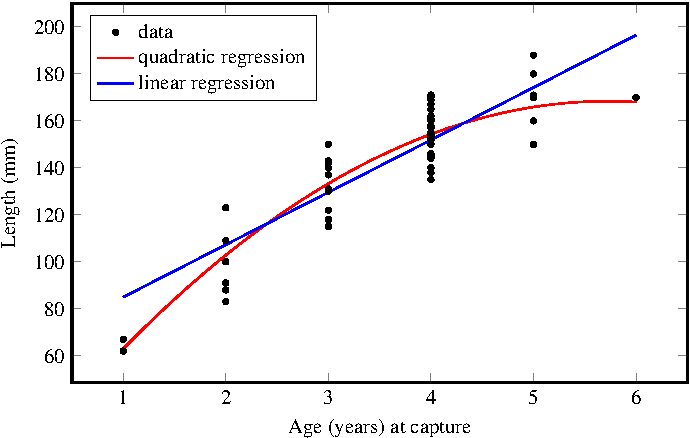
\includegraphics[scale=1.1]{image/09/bluegill.pdf}
\caption{%%
  The age versus length of $78$ bluegill sunfish.  The age of a fish
  is measured in years at the time of capture.  The length of the fish
  is measured in millimetres.  The black dots show the data in the
  file \code{bluegill.csv}.  The red curve is a graph of
  \Equation{eqn:quadratic_applications:bluegill_quadratic}.  The blue
  line is a graph of
  \Equation{eqn:quadratic_applications:bluegill_linear_regression}.
}
\label{fig:quadratic_applications:bluegill}
\end{figure}

\solutionpart{subprob:quadratic_applications:bluegill_data}
\Figure{fig:quadratic_applications:bluegill} shows a scatter plot of
the age versus length of the sampled bluegill sunfish.  The graph
shows that the dots seem to follow a straight line.  You can also
notice that the dots seem to follow a quadratic function.

\solutionpart{subprob:quadratic_applications:bluegill_regression}
You have the sums
%%
\begin{align*}
&\sum_{i=1}^n x_i^4
=
18445,
\qquad
%%
\sum_{i=1}^n x_i^3
=
4411,
\qquad
%%
\sum_{i=1}^n x_i^2
=
1093,
\qquad
%%
\sum_{i=1}^n x_i
=
283, \\[4pt]
%%
&\sum_{i=1}^n x_i^2 y_i
=
166265,
\qquad
%%
\sum_{i=1}^n x_i y_i
=
42117,
\qquad
%%
\sum_{i=1}^n y_i
=
11201.
\end{align*}
%%
The above sums can be used to calculate the determinants
%%
\begin{align*}
&D
=
689448,
\qquad
%%
D_a
=
-3253274, \\[4pt]
\qquad
%%
&D_b
=
37264190,
\qquad
%%
D_c
=
9391920.
\end{align*}
%%
The parameters $\triple{a}{b}{c}$ can be estimated as
%%
\begin{align*}
a
&=
\frac{D_a}{D}
=
\frac{-3253274}{689448}
\approx
-4.7187 \\[4pt]
%%
%%
b
&=
\frac{D_b}{D}
=
\frac{37264190}{689448}
\approx
54.0493 \\[4pt]
%%
%%
c
&=
\frac{D_c}{D}
=
\frac{9391920}{689448}
\approx
13.6224
\end{align*}
%%
and thus the given data set can be modelled as the quadratic function
%%
\begin{equation}
\label{eqn:quadratic_applications:bluegill_quadratic}
f(x)
=
-4.7187x^2 + 54.0493x + 13.6224.
\end{equation}
%%
\Figure{fig:quadratic_applications:bluegill} compares
\Equation{eqn:quadratic_applications:bluegill_quadratic} with the data
set.

\solutionpart{subprob:quadratic_applications:bluegill_coefficient_determination}
The sum of the squared errors is $\text{SSE} \approx 8920.6956$ and
the total sum of squares is $\text{TSS} \approx 44858.6795$.  Then the
regression
function~\eqref{eqn:quadratic_applications:bluegill_quadratic} has a
coefficient of determination of approximately
\[
R^2
=
1
-
\frac{\text{SSE}}{\text{TSS}}
\approx
1
-
\frac{8920.6956}{44858.6795}
\approx
0.8011.
\]

\solutionpart{subprob:quadratic_applications:bluegill_linear_regression}
Suppose that the data set can be modelled as a linear function
$g(x)$.  Then linear regression on the given data shows that the
linear regression function can be written as
%%
\begin{equation}
\label{eqn:quadratic_applications:bluegill_linear_regression}
g(x)
=
22.3123x + 62.6490
\end{equation}
%%
which is graphed in \Figure{fig:quadratic_applications:bluegill}
together with the quadratic regression function and the given data
set.  The function $g(x)$ has a Pearson correlation coefficient of
$\rho \approx 0.8573$ and hence a coefficient of determination of
$R^2 = \rho^2 \approx 0.7349$.  The quadratic regression function
$f(x)$ has a root mean square error~(RMSE) of
$R^2 \approx 10.6943$.  The corresponding value for $g(x)$ is
$R^2 \approx 12.3480$.  As you can see, quadratic regression results
in a higher value of $R^2$ than does linear regression.  Furthermore,
the function $f(x)$ has a lower RMSE value than does $g(x)$.  Based on
the values of $R^2$ and the RMSE, you may conclude that $f(x)$ is
better than $g(x)$ at modelling the given data.
\end{solution}
}{}
\end{problem}

\end{document}
